% $Id: network.tex 2 2012-09-13 23:13:00Z jbao $
\chapter{Network topology and dynamics}
\label{chap:network}

Cells initiate and control decisions like migration, proliferation or differentiation through the intricate, yet
coordinated, regulation of large gene interaction networks. 
As a consequence, there is  well orchestrated time-sequential regulation of protein pathways, resulting in and regulated by a  global change in gene expression.
Gaining insight into the necessary and suffient regulators controlling cellular decisions  is therefore difficult. 
The central questions are, how to bridge the large data set to a few regulators or key players, how does the cell come to the unique and well defined decisions despite the underlying complexity?

Systems theory points to ways how complex systems are regulated and obey common rules with respect to their organization and dynamic responses~\citep{Kauffman1993}. 
In order to tackle the complexity of such systems, 
one usually works with
an abstract
representation or a graph\footnote{Throughout the text, we use \emph{graph} and \emph{network} interchangably.} consisting of different molecules as nodes and the 
interactions among them as edges. In order to understand the
behavior of complex systems, one has to understand both
the topological and dynamical properties of networks. In this chapter, we first
introduce some graph theoretical concepts, we then investigate the dynamics and
topology of \emph{in silico} networks, finally we present a biological application.

\section{Complex networks in biology and beyond}
Biological phenomena are described in the context of a network
at all spatial and temporal scales, from the food web~\citep{Williams2000}, 
neuronal networks~\citep{White1986,Bullmore2009}, gene regulatory networks~%
\citep{Kauffman1969,Gama-Castro2008,Abdulrehman2011},
protein-protein interaction networks~\citep{Jeong2001,Stelzl2005}
to metabolic networks~\citep{Herrgaard2008}.

The study of networks dates back to the K\"onigsberg
problem from Leonhard Euler in the 18th century. The initial
problem deals with seven bridges across the river in the city
of K\"onigsberg, and the aim is to find a walk through the 
city that would cross each bridge once and only once, to which
Euler proved that there is no solution. For a long time,
graph theory remained a specialized and abstract mathematical 
discipline. Not until the publication of the first 
small-world network model~\citep{Watts1998} did people
realize that there is a class of networks, which is neither
purely random nor purely regular and can represent most of
the real-world structures, ranging from Internet, power grid
to collaboration graph of film actors, and last but not least, 
biological networks.

The study of biological networks has been largely inspired by the theoretical 
analyses of other types of networks~\citep{Barabasi2004}. In recent years, 
there is also increasing interest in the comparison between biological and
other networks. For instance, the transcriptional regulatory network of 
\emph{E. coli} is found to have a pyramid-like hierarchical 
structure, whereas the Linux kernel displays rather an inverse-pyramid
hierarchy, which is believed to be due to different design principles of the two 
systems: robustness for biological systems and cost effectiveness for 
software systems~\citep{Yan2010}.
Such findings highlight the close relationship between 
function and structure, either
the function of complex networks results from their distinct structural 
properties, or the network structure evolved to facilitate
the function.

\section{Network topology}
There are a variety of methods to determine the topology of biological
networks. For gene regulatory/transcription factor binding networks,
either the perturbation of individual components~\citep{Davidson2002} or
the large-scale identification of transcription factor-binding sites 
using chromatin immunoprecipitation followed by probing of genomic microarrays 
(ChIP-chip)~\citep{Horak2002b} or DNA sequencing (ChIP-seq)~\citep{Johnson2007} 
has been used to assemble networks.
In the case of protein-protein interaction networks, either yeast two-hybrid~%
\citep{Uetz2000,Ito2001}
or affinity purification followed by mass spectrometry~\citep{Gavin2006} is applied to 
generate large scale datasets. 
Independent of the type of the data, the study of topology in biological networks
can be assisted by
a large number of graph-theoretic topological measures.
The focus of a certain measure ranges from the local network topology to 
global topological features.

\subsection{Topological measures}
\label{sec:topology_definition}

\subsubsection{Degree and degree distribution}
The \emph{degree} (or connectivity) $k_i$ of a node $i$ is the number of edges 
connecting the node, in case of directed networks, one further distinguishes
between the incoming ($k_i^{in}$) and outgoing degree ($k_i^{out}$). Then the total 
degree is defined as $k_i = k_i^{out} + k_i^{in}$. A list of the node degrees 
of a network is called the \emph{degree sequence}.

The \emph{degree distribution} $P(k)$, or the fraction of nodes in the graph 
$G$ having degree $k$, is probably the most basic topological 
characterization of a graph. It has been shown that the degree distribution of
a neuronal network determines its global oscillatory state~\citep{Roxin2011}, 
and by assuming linear dynamics at the individual nodes, 
the number of driver nodes in a network is determined mainly by the 
network's degree distribution~\citep{Liu2011}.

\subsubsection{Shortest path and betweenness}
\label{sec:shortest_path}
\emph{Shortest paths} $d_{ij}$ from node $i$ to node $j$ play an important 
role in the transport and communication 
within a network. Although highly efficient algorithm exists to perform
route planning such as in Google Maps~\citep{Sanders2005}, common algorithms
for calculating shortest paths are Dijkstra's algorithm~\citep{Dijkstra1959} for weighted networks
and the breadth-first search~\citep{West2000} for unweighted networks.

An extension of the shortest path is a measure of the importance of a given 
node defined by the sum of the fraction of all-pairs shortest paths that pass 
through it, or the 
\emph{betweenness} $b_i$ of a node $i$~\citep{Freeman1977} is given by
\begin{equation}
b_i = \sum_{s,t \in N} \frac{\sigma(s,t|i)}{\sigma(s,t)},
\end{equation}
where $N$ is the set of nodes, $\sigma(s,t)$ is the number of shortest paths 
between node $s$ and $t$, and $\sigma(s,t|i)$ is the number of those paths 
passing through the node $i$ other than $s$ and $t$.

\subsubsection{Motif}
A \emph{network motif} $M$ is a pattern of interconnections occurring in complex 
networks at a number that is significantly higher than those in randomized 
networks~\citep{Milo2002,Shen-Orr2002}. The statistical significance of M is 
then described by the $Z$-score, defined as
\begin{equation}
Z_M = \frac{n_M - \langle n_M^{rand} \rangle}{\sigma_{n_M^{rand}}},
\end{equation}
where $n_M$ is the number of times the subgraph $M$ appears in $G$, and 
$\langle n_M^{rand} \rangle$ and $\sigma_{n_M^{rand}}$ are, respectively, 
the mean and 
standard deviation of the number of appearances in the randomized network ensemble.
Motifs have been strongly linked to the information processing in networks, 
for example, the incoherent feedforward loop was shown to be able to detect
fold change in the input signal~\citep{Goentoro2009}.

\subsubsection{Community}
A \emph{network community} or module is a subnetwork with many edges joining
nodes of the same cluster and comparatively few edges joining nodes of 
different clusters. Since such communities can be considered as fairly 
independent compartments of a graph, they are usually also assigned 
a similar function, e. g., individual tissues or organs in the human body,
pathways within the cellular signal transduction network, a group of people
with common interest within the social network~%
\citep{Fortunato2010,Newman2012}.

There is now a zoo of algorithms to detect network communities, probably one
of the most influential methods is the algorithm proposed by \cite{Girvan2002},
which aims at the identification of edges lying between communities and their 
successive removal, a procedure that after some iterations
leads to the isolation of the communities. Most recently, \cite{Ahn2010b} 
suggested that each node in a network can in principle belong to more than 
one functional group, they therefore reinvented the definition of communities 
as groups of links rather than nodes and demonstrated this approach can uncover
the natural overlap while revealing hierarchical organization of the network.

\subsection{Scale-free networks}
\label{sec:scale_free}
Together with the small-world network model, the scale-free network model~%
\citep{Barabasi1999} has
also attracted much attention in the research community.~% 
\footnote{We think this topic deserves its own section and we also discuss
the relevance of scale-free networks in our results later.}
The basic idea of 
how a scale-free network and its power-law degree distribution come into
existence is called preferential attachment. In other words, at each time
step of a growing network, a new node is added to a certain node in the 
network based on the probability that is proportional to the degree of the
given node, i.e. strongly connected nodes will get more and more connections, or
popular nodes will be even more attractive. Such a model is able to reproduce
the power-law degree distribution observed in scale-free networks.

However, recent years have seen a critical assessment of the original 
scale-free model. On the one hand, several rigorous statistical analyses~%
\citep{Clauset2009,Khanin2006a} have shown that methods used to fit power-laws, such as 
least-squares, can produce substantially inaccurate estimates of the 
parameters. The authors concluded that in general the cumulative distribution
function is more robust than the probability density function against 
fluctuations due to finite sample sizes, especially in the tail of the 
distribution. It is also extremely difficult to distinguish between
the log-normal and power-law distribution. These results cast doubt on the
validity of most empirical characterization of power-law degree distribution
and the significance of classifying scale-free networks according to such
degree distributions.

On the other hand, there is now increasing evidence that mechanisms other than
preferential attachment can also lead to the empirical power-law degree 
distribution~\citep{Caldarelli2002}. For instance, a model of unspecific 
binding between proteins results exactly in a scale-free protein-protein 
interaction network~\citep{Deeds2006}.

\section{Network dynamics}
Imagine the scene of fireworks, the beauty lies exactly in the whole sequence 
of explosive events. When you try to snap a shot, it is possible that you end up with
a black sky. Even if you are able to capture the highlight, 
you have still 
effectively missed certain information, such as how the 
visual pattern developed,
what is the interval between consecutive illuminations. 
On the other extreme, one also loses information when making
a long-exposure photograph out of the whole sequence.
The same holds in the
study of complex networks, if we want to understand the behavior of networks,
we always have to study their dynamics at an appropriate time scale, 
rather than simply in a static context.

Here the network dynamics refers specifically to the dynamic response of the 
gene regulatory network or transcriptome. 
Various technologies have been 
developed to deduce and quantify the 
transcriptome, including hybridization- 
or sequence-based approaches~\citep{Wang2009}. 
Although not the focus of this thesis, the recently developed
RNA-Seq method is an attractive sequence-based approach.
In contrast,
hybridization-based approaches include the classical microarray
technology, which takes advantage of hybridization properties 
of nucleic acids and uses complementary molecules (probes) attached to a solid 
surface 
(chip) to measure the quantity of specific nucleic acid transcripts of 
interest that are present in a sample. A specialized scanner is used to 
measure the amount of hybridized target at each probe, which is reported as an 
intensity~\citep{Gentleman2005}. This intensity value is then interpreted as a
proxy for the level of gene expression. In order to characterize the global 
gene expression given a certain stimulus over time, one can perform the 
hybridization at multiple time points. The ultimate gene expression data are
thus multidimensional time series. 



We provide two distinct 
perspectives of viewing the gene expression time series.
In the following, we first deal with ranking the 
single gene dynamics within the same experimental condition by multidimensional
scaling.
As an alternative, we discuss in \ref{sec:full_reduced} a likelihood ratio test of kinetic profiles between two conditions
by fitting a linear model to the time series.

\subsection{Dimensionality reduction}
Dimensionality reduction is the transformation of high-dimensional data into 
a meaningful representation of reduced dimensionality~\citep{Maaten2009}, 
which is easy to both visualize and interpret. There is a whole spectrum of linear
and nonlinear dimensionality reduction algorithms 
(\ref{fig:dimension_reduction}). In this work, we heavily 
focus on a variant of Euclidean distance based multidimensional 
scaling (MDS), which is similar to principal component analysis (PCA)%
~\citep{Haerdle2003},
but more flexible and intuitive. We also evaluate the performance of MDS in comparison to 
PCA in the following.

\begin{figure}[!ht]
\begin{center}
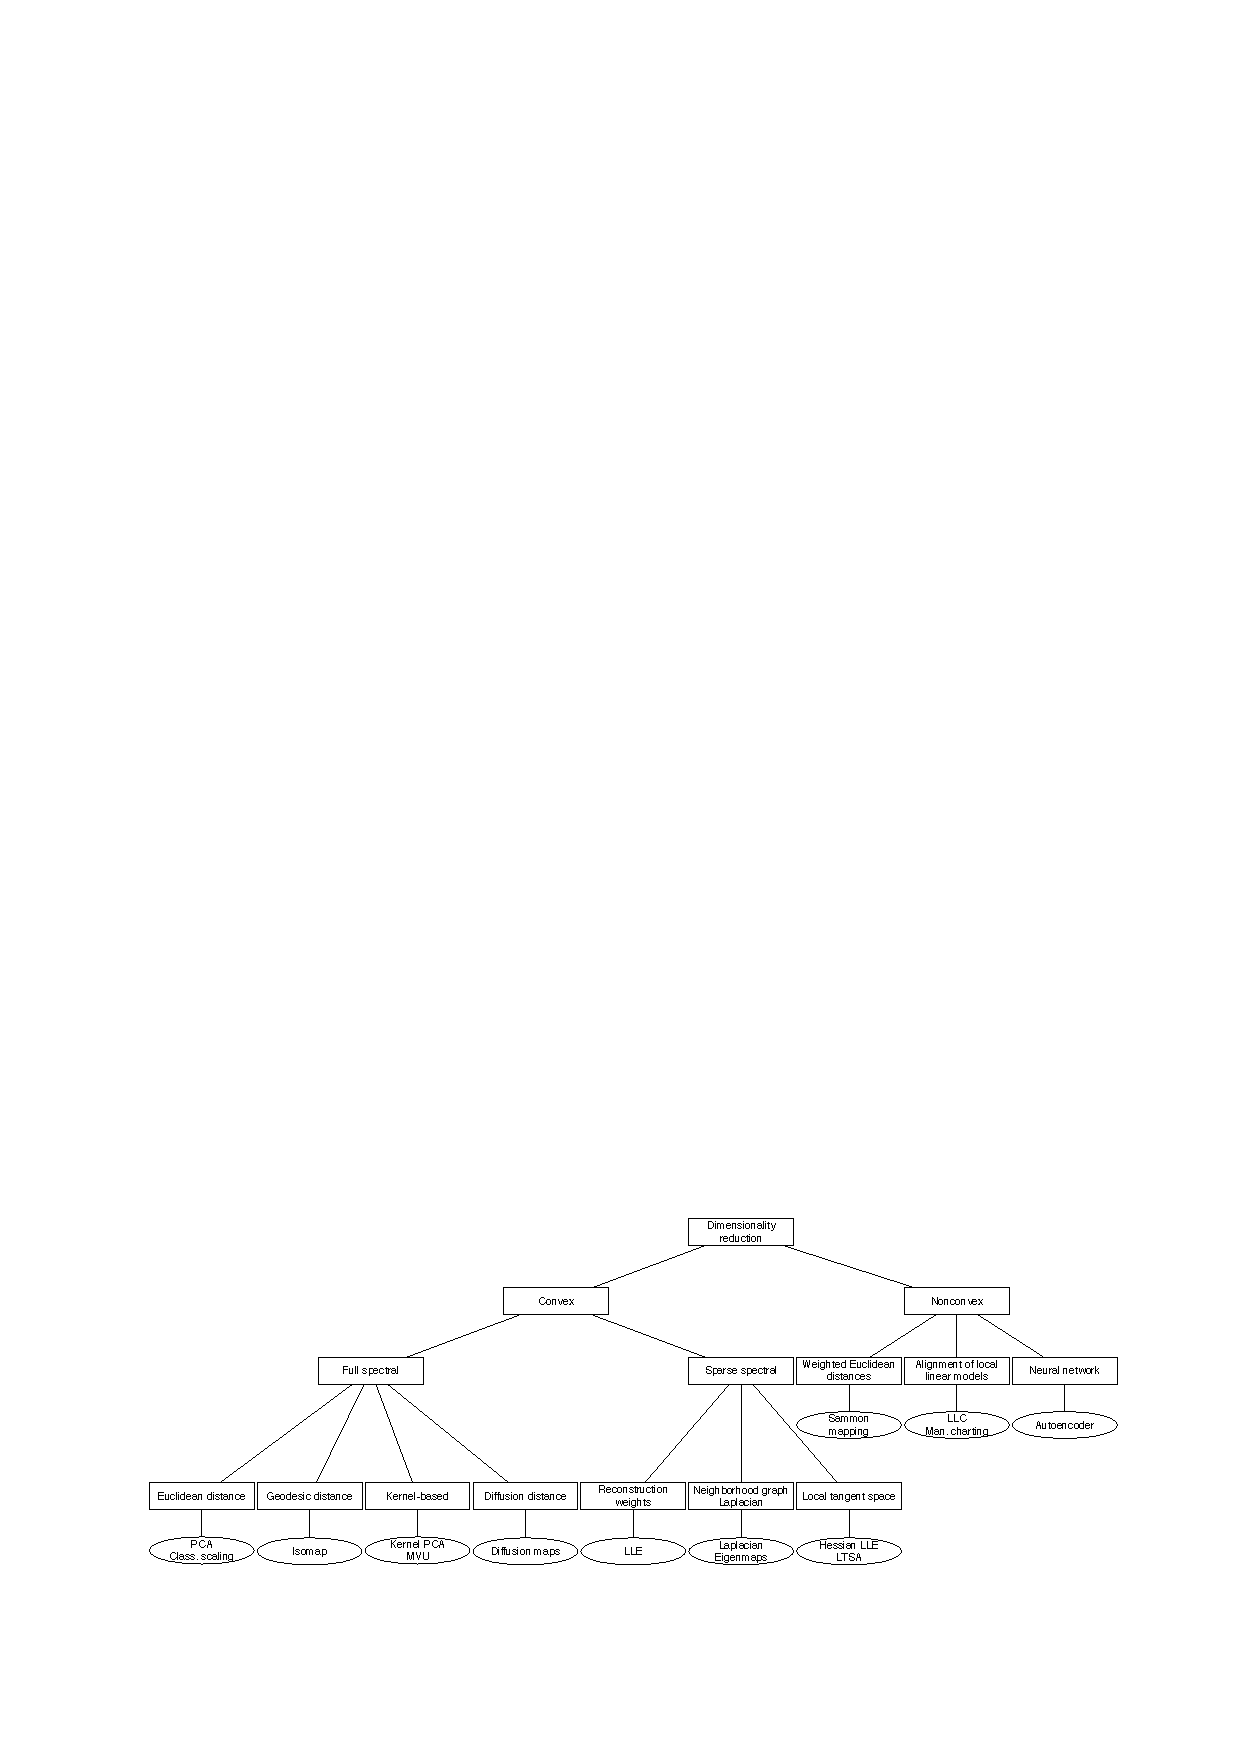
\includegraphics[width=\textwidth]{network/fig/dimension_reduction.pdf}
\end{center}
\caption[Dimensionality reduction algorithms]{
{\bf The taxonomy of dimensionality reduction algorithms.}
A non-exhaustive overview of diverse dimensionality reduction
techniques, taken from \cite{Maaten2009}.
}
\label{fig:dimension_reduction}
\end{figure}

\subsubsection{Multidimensional scaling}
\label{sec:mds}
Multidimensional scaling (MDS) is a family of algorithms that produces a spatial
representation of the dissimilarities between a number of entities $x_l^i \in 
\boldsymbol{X}_{n \times q}$ in $q$-dimensional space. In 
principle, MDS takes as input a symmetric $n \times n$ matrix 
\begin{equation}
  \boldsymbol{D} = \sqrt{\sum_{l=1}^q (x_l^i - x_l^j)^2}_{\substack{i \neq j,\\
    i,j=1...n}},
\end{equation}
which
describes the dissimilarities between the high-dimensional
entities. Those entities
are then represented by points in a low-dimensional space $\hat{x}_l^i \in 
\hat{\boldsymbol{X}}_{n \times d}$ ($d$ usually equals $2$ or
$3$ for ease of visualization), which are positioned
such that the pairwise distances between them 
\begin{equation}
  \hat{\boldsymbol{D}} = \sqrt{\sum_{l=1}^d (\hat{x}_l^i - \hat{x}_l^j)^2}_{\substack{
    i \neq j,\\i,j=1...n}}
\end{equation}
reflect as closely as possible  
the original
dissimilarities between the entities. 
The optimization of the spatial configuration can be realized by the 
minimization of different stress functions.
We applied
here the HiT-MDS-2 algorithm (\citealp{Strickert2009}), where the
Pearson correlation of the original and the reconstructed distances 

\begin{equation}
  r(\boldsymbol{D}, \hat{\boldsymbol{D}}) = \frac{\sum_{i \neq j}^n (d_{ij} - \mu_{\boldsymbol{D}}
    ) \cdot (\hat{d}_{ij} - 
    \mu_{\hat{\boldsymbol{D}}})}{\sqrt{\sum_{i \neq j}^n (d_{ij} - \mu_{\boldsymbol{D}})^2} 
    \cdot \sqrt{
    \sum_{i \neq j}^n (\hat{d}_{ij} - \mu_{\hat{\boldsymbol{D}}})^2}}
  \label{eq:dist_corr}
\end{equation}
is defined as the negated stress function and is maximized using a gradient descent approach.
Particularly, $\boldsymbol{D} = (d_{ij})_{i,j=1...n}$ is Euclidean distance matrix of the
gene expression time series, and $\hat{\boldsymbol{D}} = (\hat{d}_{ij})_{i,j=1...n}$ 
is the 
Euclidean distance matrix of the reconstructed low-dimensional points. 
$\mu_{\boldsymbol{D}}$ and $\mu_{\hat{\boldsymbol{D}}}$ are the mean of matrix $\boldsymbol{D}$
and $\hat{\boldsymbol{D}}$ respectively.
\begin{eqnarray}
  \mu_{\boldsymbol{D}} = \frac{2}{n (n-1)} \sum_{i<j}^N d_{ij},\\
  \mu_{\hat{\boldsymbol{D}}} = \frac{2}{n (n-1)} \sum_{i<j}^N \hat{d}_{ij}.
\end{eqnarray}
%A stress function 
%\begin{equation}
%  s = -r(\boldsymbol{D}, \hat{\boldsymbol{D}})
%\end{equation}
%is minimized by gradient descent.
Throughout this work, the number of optimization cycles is fixed to be $100$.
Since any reflection or rotation of the low-dimensional point configuration
remains a valid solution of MDS,
we centered the final configuration, normalized it by the largest dimension variance,
and rotated it by Principal Component Analysis to generate a unique 
representation of the low-dimensional configuration.

\subsubsection{Performance of multidimensional scaling}
Taking the time-resolved gene expression profiles of hepatocyte growth factor
stimulated keratinocytes as an example, we projected the time series onto a 
two-dimensional space by different algorithms and assessed their performance
by calculating the correlation between the original and reconstructed distance
matrices (\ref{eq:dist_corr}).

While the correlation of distances by PCA (\ref{fig:svd-mds} A) is 0.89, two 
realizations of the HiT-MDS-2 algorithm show a correlation coefficient around 
0.98 (\ref{fig:svd-mds} C,D). Although this is slightly lower than the correlation of a recently 
proposed algorithm (\ref{fig:svd-mds} B), it clearly outperforms PCA. The 
better performance of the SVD-MDS algorithm~\citep{Becavin2011} results from
the fact that it initializes the spatial configuration with PCA instead of 
random guess, thus already starts from a relatively good solution of MDS and
avoids being stuck in local minima.

\begin{figure}[!ht]
\centering
%\begin{narrow}{-0.5in}{-0.5in}
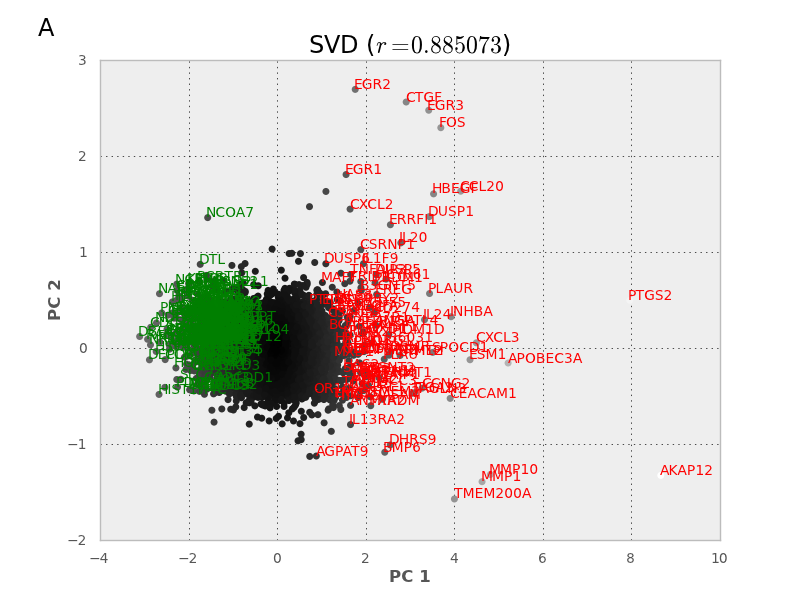
\includegraphics[width=0.45\textwidth]{svd.png}
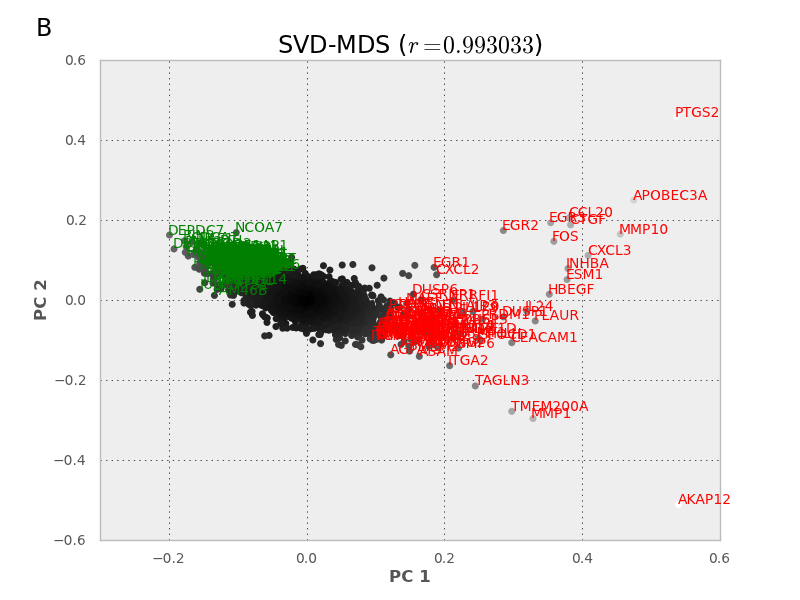
\includegraphics[width=0.45\textwidth]{svd-mds.png}\\
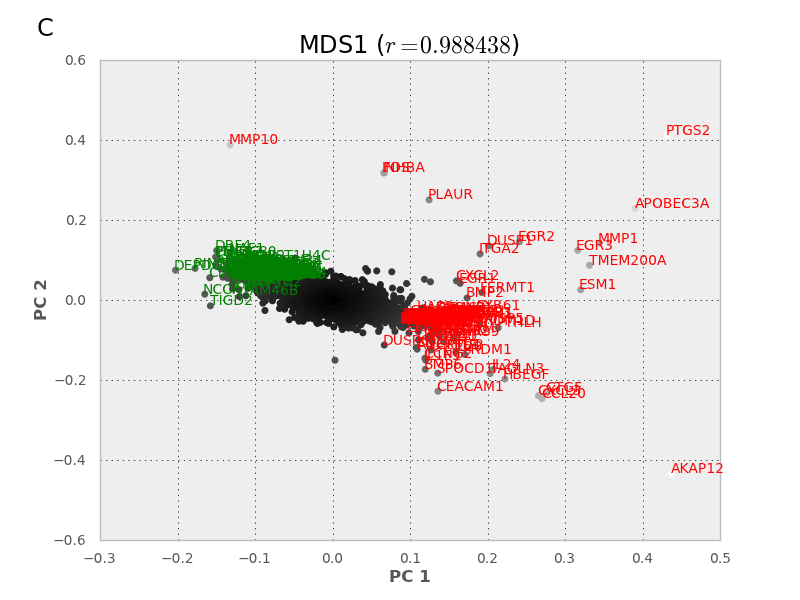
\includegraphics[width=0.45\textwidth]{mds1.png}
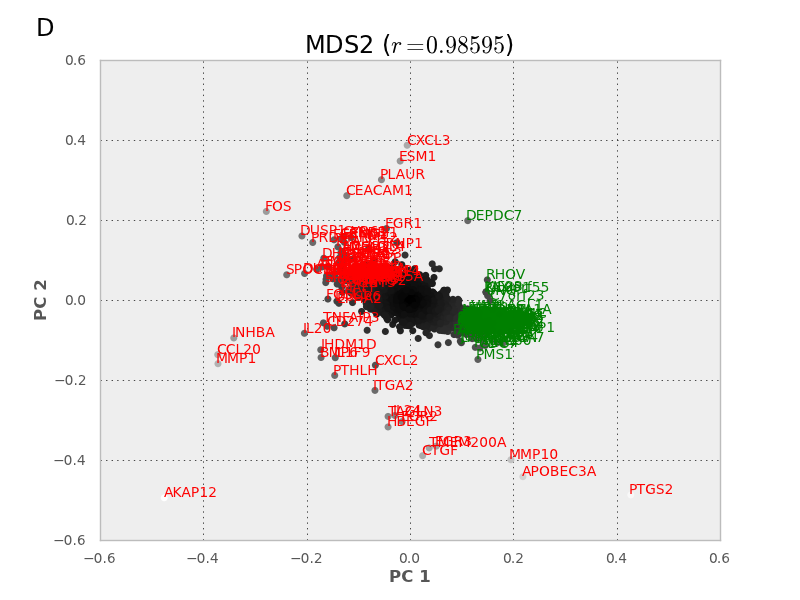
\includegraphics[width=0.45\textwidth]{mds2.png}
%\end{narrow}
\caption[Performance of the MDS algorithm]{
{\bf Comparison of SVD and MDS algorithms.}
(A) Singular 
value decomposition (SVD), which is the basis of PCA. (B) SVD-MDS
proposed by \citealp{Becavin2011}, which first makes use of
SVD to initialize the low-dimensional configuration in MDS.
(C,D) MDS run with two different random initial 
configurations. $r$ indicates the correlation between the
original and the reconstructed distance matrices (see also
\ref{sec:mds}). 
Data are taken from the 8h time course of primary human keratinocytes 
stimulated with hepatocyte growth factor (\cite{Busch2008}, 
ArrayExpress accession number E-TABM-440),
red and green labels represent up- and 
down-regulated genes with an average $\log_2$ fold expression 
$> 0.5$. }
\label{fig:svd-mds}
\end{figure}

\subsubsection{Response strength metric}
\label{sec:response_strength}
In order to quantify the response strength of a single gene, we make use of 
MDS, namely by fitting a skewed Gaussian distribution (\citealp{Azzalini2003}) 
to the 2-D projection
of gene expression time series and assigning a $p$-value to each
gene according to its probability of being drawn from the fitted distribution.
We further take the negative logarithmic of the $p$-values as the response
strength metric. In so doing, a gene located at the periphery of the MDS
projection has a small $p$-value and thus a large response strength, whereas
central genes have small response strengths.

A multivariate skewed Gaussian distribution is defined as follows, suppose
$X$ is a $d$-dimensional random variable with a probability density function
\begin{equation}
f(X) = 2 \phi_d (X;\Omega) \ \Phi(\alpha^{\mathrm{T}} X), \quad X \in \mathbb{R}^d,
\label{eq:sn}
\end{equation}
where $\phi_d(X;\Omega)$ is the $N_d(0,\Omega)$ normal density function at $X$
with the correlation matrix $\Omega$, $\Phi(\alpha^{\mathrm{T}} X)$ is the 
cumulative distribution function of $N(0,1)$ evaluated at $\alpha^{\mathrm{T}} X$.
$\alpha$ is the shape parameter since when $\alpha=0$, \ref{eq:sn} becomes
the regular normal probability density function again. $X$ can be further
linear transformed to
\[
Y = \xi + \omega X
\]
to include the location and scale parameter, $\xi$ and $\omega$ respectively.

Fitting of the skewed Gaussian distribution is performed with
the maximum likelihood method as implemented in the 
\texttt{R}
library \texttt{sn}.

\subsection{Heavy-tailed response distribution}

\begin{figure}[!ht]
\begin{center}
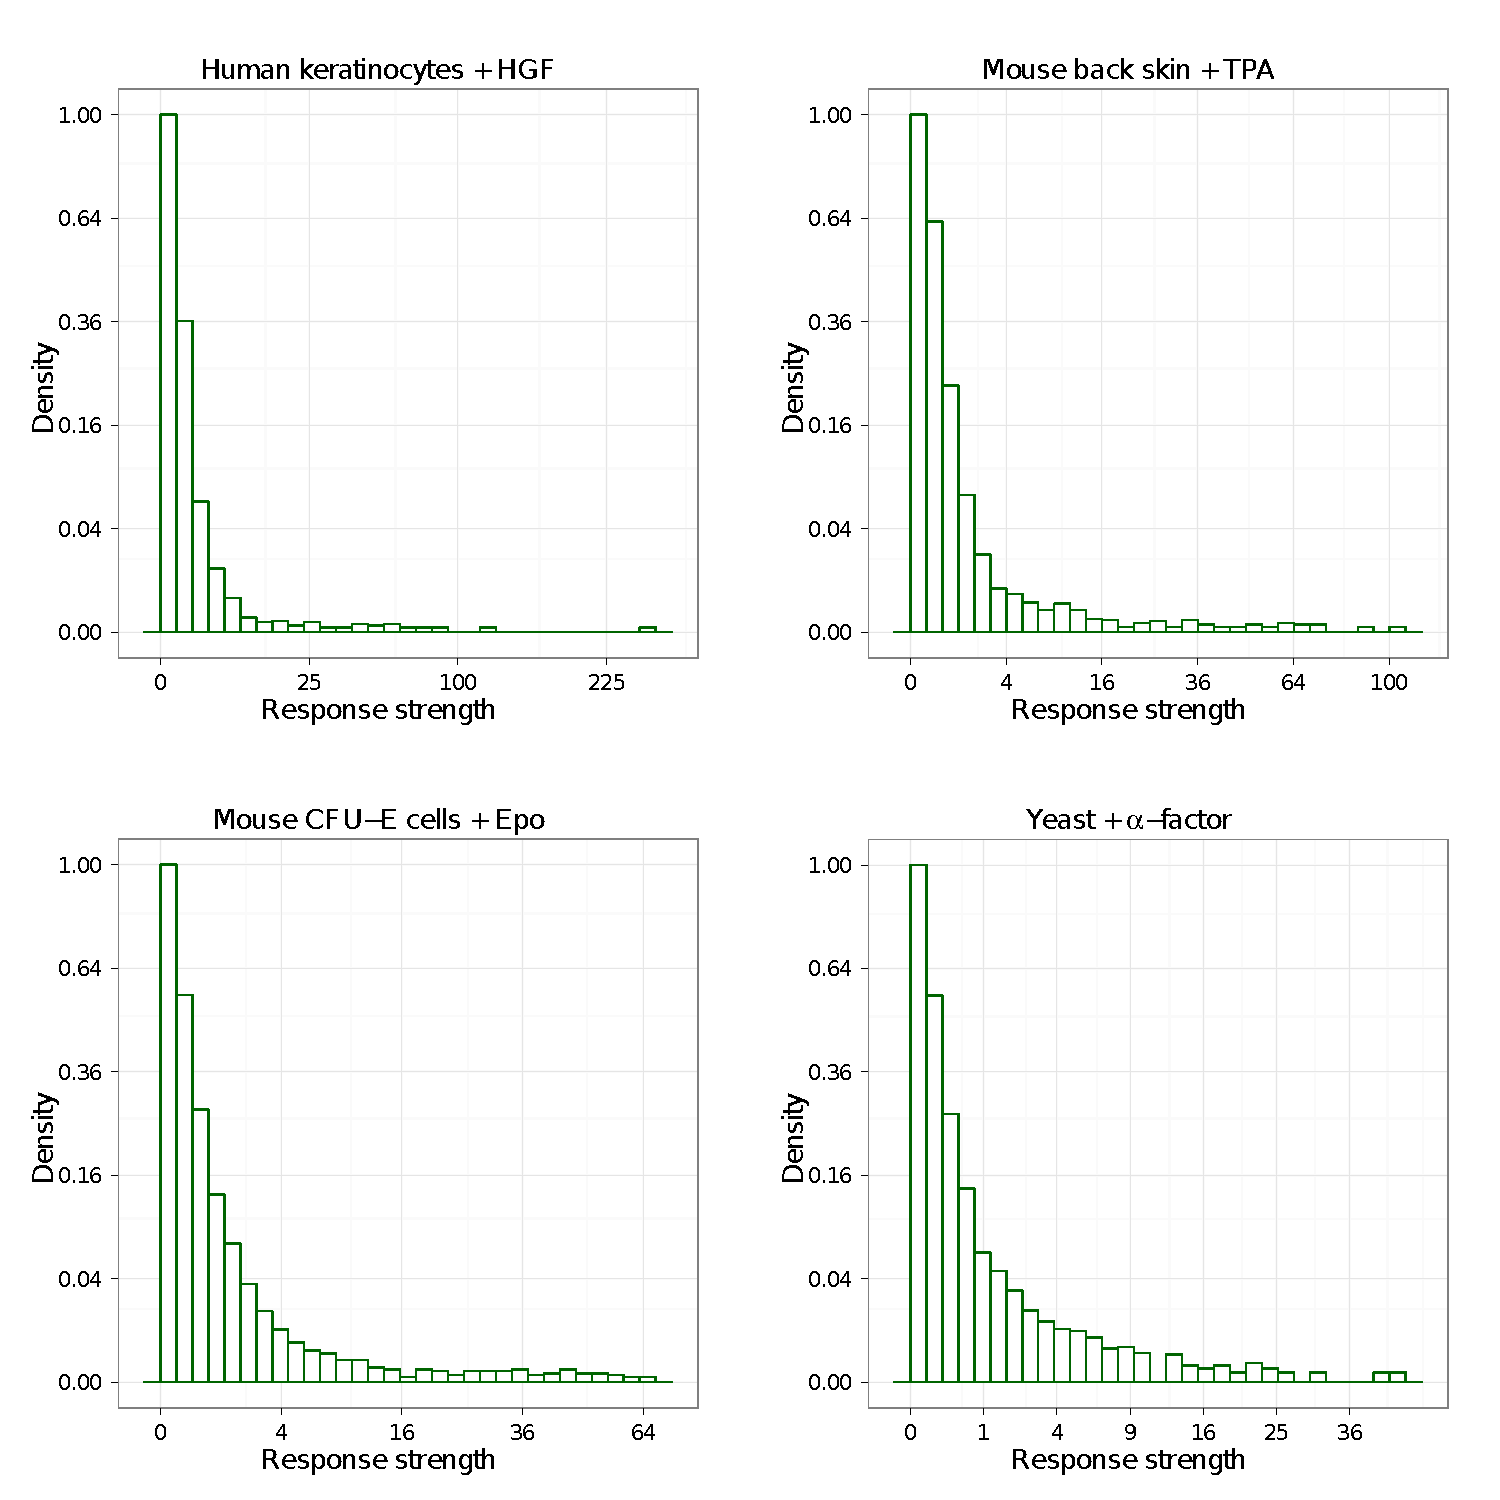
\includegraphics[width=\textwidth]{network/fig/response_all.pdf}
\end{center}
\caption[Heavy-tail distribution of gene response strength]{
{\bf Distribution of gene response strength in different
cell types under different stimulation.}
Gene response strengths are calculated as described in 
\ref{sec:response_strength}, the maximum of each distribution
is normalized to 1. Datasets used in this plot include 
primary human keratinocytes 
stimulated with hepatocyte growth factor (ArrayExpress database 
\texttt{http://www.ebi.ac.uk/arrayexpress/},
accession number E-TABM-440); Mouse skin cells stimulated with TPA,
an inducer of skin inflammation (provided by the author); 
CFU-E cells from mouse fetal livers stimulated
with Epo (GEO database \texttt{http://www.ncbi.nlm.nih.gov/geo/}, accession
number GSE26151); yeast cells synchronized with 
$\alpha$-factor to study the cell cycle
\\(\texttt{http://genome-www.stanford.edu/cellcycle/data/rawdata/combined.txt}).
}
\label{fig:response_strength}
\end{figure}

With the help of the $p$-value based response strength score,
we can easily assess both the significance of the regulation of
a certain gene and the general response pattern of all genes
in a regulatory network.
Interesting questions include the transcriptome response
similarity between different
experimental setups (\ref{fig:response_strength}). 
For example, in the case of transcripts
profiled in primary human keratinocytes under the stimulation of 
hepatocyte growth factor (HGF)~\citep{Busch2008}, we found the distribution of response
strengths has a long tail, indicating that 
only few genes are strongly induced by a certain stimulus, while the majority 
are barely regulated. This long-tail response strength
distribution is also observed in other cell types with various stimuli.
Among them are yeast cells that undergo cell cycles when synchronized by 
$\alpha$-factor~\citep{Spellman1998,Cho1998}, mouse skin cells stimulated with TPA,
an inducer of skin inflammation~\citep{Riehl2010} and erythrocyte progenitor
(CFU-E) cells from the mouse fetal liver stimulated with erythropoietin (Epo)~\citep{Bachmann2011}. 

None of the response distributions fits well with any theoretical 
Gaussian, power-law, exponential, log-normal or Weibull distributions, with the closest one being power-law or log-normal
distribution up to a certain range (\ref{fig:response_fit}). 
Nevertheless, the response distributions from various 
biological systems do share the same shape between each 
other (\ref{fig:response_qqplot}). Taken together, gene
responses in various systems are indeed heavy-tailed distributed, with few
genes strongly regulated and the majority only moderately
regulated. However, the response strength itself does not exactly 
follow the power-law distribution,
which underlines again the necessity of assessing power-law
distributions on empirical data within a rigorous statistical
framework~\citep{Clauset2009}.

\begin{figure}[!ht]
\begin{center}
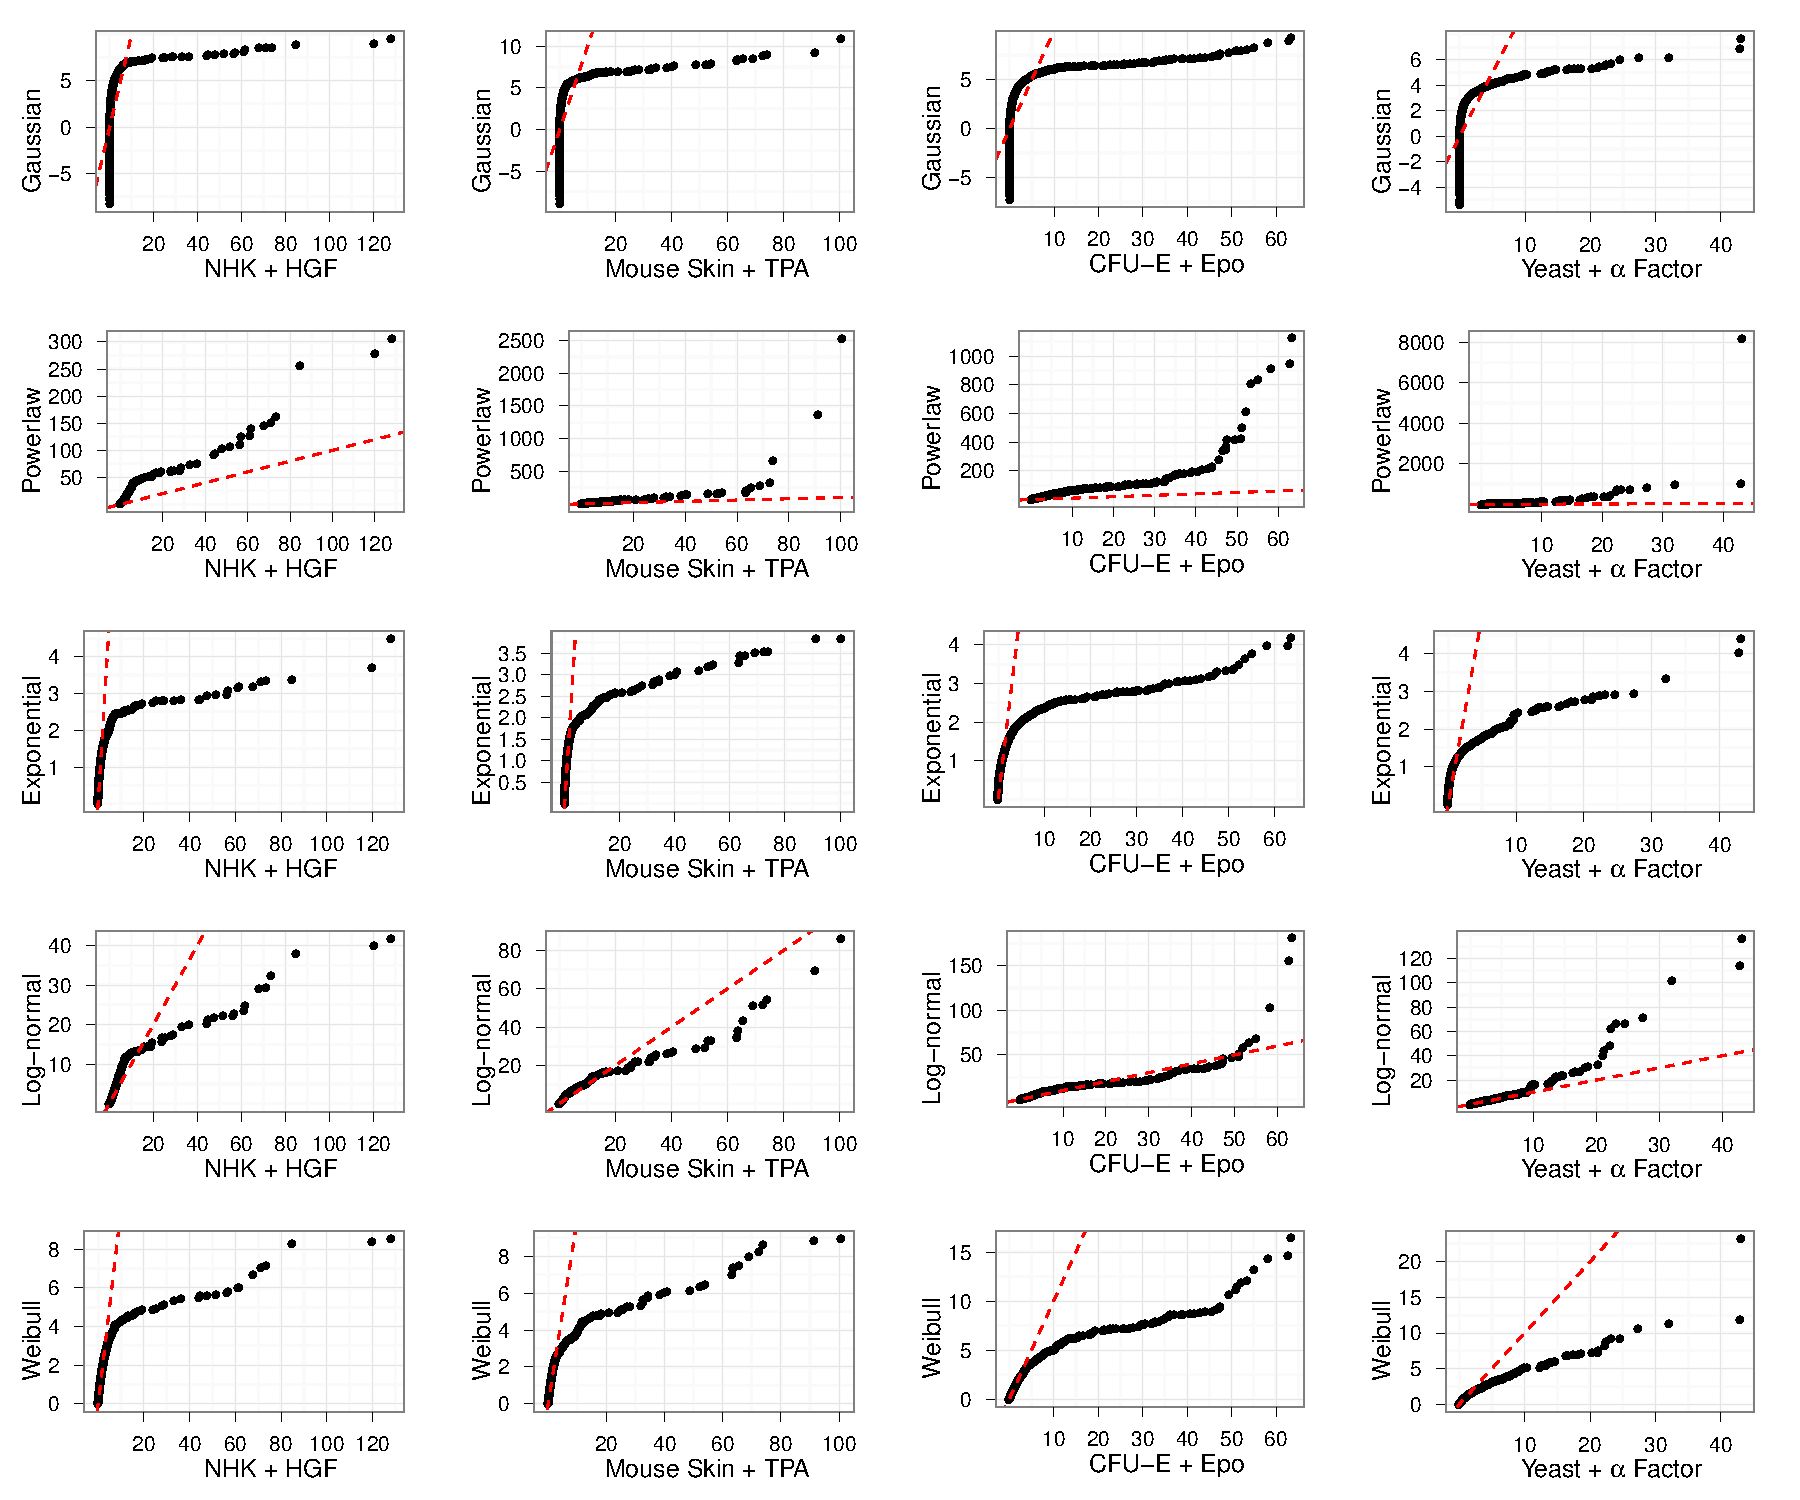
\includegraphics[width=\textwidth]{network/fig/response_fit.pdf}
\end{center}
\caption[Comparison of gene response distributions with
theoretical distributions]{
{\bf Comparison of gene response distributions with 
different theoretical distributions using the quantile-%
quantile plot.}
Biological datasets are the same as in 
\ref{fig:response_strength}, red dashed lines have a slope
of 1 and indicate identity, theoretical distributions 
include Gaussian, power-law, exponential, log-normal and
Weibull distribution~\citep{Clauset2009}.
}
\label{fig:response_fit}
\end{figure}

\begin{figure}[!ht]
\begin{center}
\includegraphics[width=\textwidth]{network/fig/response_qqplot.pdf}
\end{center}
\caption[Comparison of gene response distributions]{
{\bf Pairwise comparison of gene response distributions with 
each other using the quantile-%
quantile plot.} 
Biological datasets are the same as in 
\ref{fig:response_strength}, red dashed lines have a slope
of 1 and indicate identity, the maximal response strength
in each dataset is normalized to 1.
}
\label{fig:response_qqplot}
\end{figure}

The finding of the heavy-tailed response distribution provides a theoretical
proof of various microarray normalization schemes, since it is often assumed
that the majority of 
genes are not differentially regulated or the number of upregulated genes 
roughly equals the number of downregulated genes~\citep{Do2006}.
Furthermore, it is known that the structures of
regulatory networks in various species are highly conserved~\citep{Brown2007}, 
we thus hypothesize that this
universally invariant transcriptome response pattern results from the generic
topological features of the gene regulatory networks. To test this hypothesis,
the following questions also
arise, namely what distinguishes 
between the strongly and weakly responding genes? How is phenotype encoded 
in the gene network?


\section{Gene response and connectivity}
In order to decipher the interplay between gene network 
dynamics and topology \emph{in silico}, 
we need a modelling framework that can ideally translate
network connectivity to dynamics in a biologically plausible
manner. We chose a general model that
expresses the dynamics of a target gene as a function of the
activity of its upstream transcriptional regulators. This
activity is further determined, according to the principles
of statistical thermodynamics, by the joint binding probability
of each regulating gene.
This model was also implemented in the simulation tool
\texttt{GeneNetWeaver}~\citep{Schaffter2011} and has proven
to be a useful benchmark model in the assessment of
diverse reverse-engineering algorithms.
Through the model simulation, 
we observed that the response strength of the gene network
is primarily determined by its topology. This topological
determinant is more dominant in large and scale-free-like 
networks, it is also 
visible in various biological networks.

\subsection{Synthetic \emph{in silico} networks}
We constructed various \emph{in silico}
network models, which span between the theoretically 
well-established ones (random graph) and biologically
motivated ones (scale-free and bow-tie network).

\subsubsection{Topology}
\begin{itemize}
\item Random: an Erd\H{o}s-R\'enyi graph (\citealp{Erdos1959}) is generated with a probability
  $0.003$ to choose each of the possible edges.
\item Uniform: network with uniform in- and out-degree distributions $k_{in,out} \in 
  \{0,1,...,11\}$ is constructed 
  with the configuration model (\citealp{Newman2001}). 
  In short, each node $i$ has a desired degree $k_i$, 
  so we imagine that each node has $k_i$ edge ``stubs'' attached to it. Edges are 
  then assigned by randomly choosing two stubs and drawing an edge between them.
\item Small-world: a small-world graph  
according to the 
Watts-Strogatz model~\citep{Watts1998} is generated, 
each node is connected
to 5 nearest neighbors in the ring topology and each edge
has a rewiring probability of 0.1. In the end, the 
undirected small-world graph is converted to a directed
graph by randomly assigning edge directions.
\item Scale-free: similar to the case of uniform networks,
except that Poisson in-degree (with $\lambda = 3$) and power-law 
  out-degree distributions ($P(k) = k^{-2.5}$) are assumed as the input
  to the configuration model.
\item Bow-tie: two growing network (GN) graphs 
  (\citealp{Krapivsky2001}) of equal size are first 
  constructed by adding nodes one at a time with an edge to one existing node, 
  which results in two directed trees. With redirection probability $0.1$ the edge
  connects the additional node with the successor node of the random selected target
  node instead of the target node itself. One of the trees is then reversed and 
  concatenated to the other one through the root nodes, such that the resulting
  graph is of the multiple-input multiple-output type.
\end{itemize}
All \emph{ad hoc} parameters are chosen in order to keep the total number of connections
and the incoming degree of a node manageable in the numerical simulation.
The network size is varied from 10 to 1000 nodes and are generated with the Python package NetworkX 
(\citealp{Hagberg2008}), they are further made sure to be connected.

\subsubsection{Dynamics}
We adapted a thermodynamical gene network model 
(\citealp{Schilstra2002,Marbach2010,Schaffter2011}),
which takes into account the combinatorial control of transcription factors. 
Precisely, the 
gene expression dynamics is defined by 
\begin{equation}
  \dot{x_i}(t) = m_i \cdot f_i(x_j(t)) - d_i \cdot x_i(t), 
\label{eq:gnw_model}
\end{equation}
where $x_i(t)$ denotes the expression level of gene $i$ at time $t$, 
$m_i$ is the 
maximum transcription rate, and $d_i$ the mRNA degradation rate. $f_i(\cdot)$
is the activation function of gene $i$, it depends on the expression level of 
all the input onto gene $i$ at time $t$, $x_j(t)$ and is the sum of relative 
activations for
different binding states. In general, for $N$ input genes, there are altogether
$2^N$ possible binding states and
\begin{equation}
  \displaystyle f_i(x_j) = \sum_{m=0}^{2^N-1} \alpha_m \theta_m,
\end{equation}
$m$ can be interpreted as an $N$-digit binary number (with padding $0$s) 
and represents one particular binding state, with the $i$-th
digit indicating the binding state of the $i$-th input gene, namely $0$ for unbound
and $1$ for bound. $\alpha_m$ is the relative activation of state $m$,
$\theta_m$ is the joint probability of state $m$: 
\begin{equation}
  \theta_{m} = \prod_j \frac{x_j^{n_{ij}}}{k_{ij}^{n_{ij}}+x_j^{n_{ij}}}
    \cdot \prod_k \frac{k_k^{n_{ik}}}{k_{ik}^{n_{ik}}+x_k^{n_{ik}}}
\end{equation}
where the probability of a single transcription factor bound to the gene is 
modelled by a Hill function,
$n$ is the Hill coefficient and $k$ is the dissociation constant, at which the
saturation is half-maximal or the transcription factor is bound $50\%$ of the time.
$x_j$ are the bound transcription factors of $x_i$ and $x_k$ the unbound ones.

Time series are simulated by first finding the steady state, where the absolute
concentration change is smaller than $10^{-5} + 10^{-3} \cdot x_i$ for each gene
or the maximal time of $500$ is exceeded. Afterwards, the basal activation $\alpha_0$
is randomly perturbed and the gene expression dynamics is simulated for a total
time of $200$ with $10$ as the time interval and the
steady state as the initial condition.

%\CC{} code of the model adapted from GeneNetWeaver (\citealp{Schaffter2011})
%is available upon request.

\subsubsection{Rewiring and change of parameters}
In order to compare the influence of both topology and 
kinetic parameters on 
the network response, we changed the network topology by rewiring edges and 
the kinetic parameters $m_i, d_i$ (\ref{eq:gnw_model}) of a gene $i$ 
respectively (\ref{fig:rewiring_scheme}). The
network response strengths before and afterwards were then compared by
calculating the Pearson correlation. More specifically, in the case of 
rewiring, the list of target nodes is randomly permuted and assigned to the
source nodes to form new edges. 
In such a way, the total number of edges
remains the same after rewiring. 
Topology-related parameters $\alpha, k, n$ are
then regenerated, but kinetic parameters remain the same. 
When changing the model parameters of individual genes, we fixed the network
topology, but changed both the intrinsic response of individual genes and 
the connection strength by tuning the kinetic and topological parameters 
respectively.

\subsubsection{Stimulation scheme}
Except otherwise noted, the pertubation factors applied on 
each node are drawn from the normal distribution 
$\mathcal{N}(0,0.33)$ (\emph{norm}) according to the 
implementation in \texttt{GeneNetWeaver}. In order to test the 
effect of perturbation on network dynamics, we also compared 
two alternative
perturbation strategies. In the \emph{max} perturbation, all basal activation
rates are clamped to the maximal value of 1 at the beginning of the
simulation. The ranked perturbation (\emph{rank}) is applied
to circumvent the fact that hub genes are usually hardly 
perturbed under the \emph{norm} condition, which results from
the small amount of hubs in a network. In the \emph{rank}
perturbation, the
perturbation factor is proportional to the degree of a node, with an empirical scaling 
factor of 0.01. Therefore, hub nodes are perturbed more strongly and 
sparsely connected nodes are only moderately perturbed.

\begin{figure}[!ht]
\begin{center}
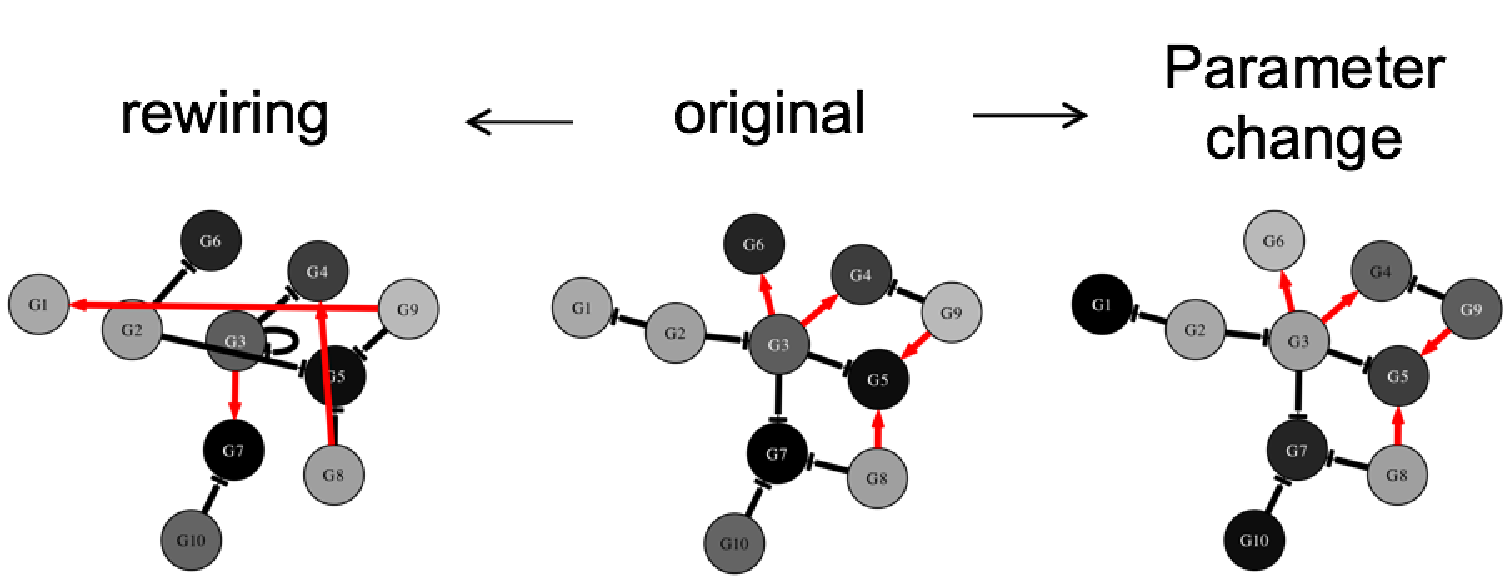
\includegraphics[width=\textwidth]{rewiring_scheme.pdf}
\end{center}
\caption[Schematic view of network rewiring and kinetic parameter change]{
{\bf Schematic view of network rewiring and change of kinetic parameters.} 
Black edges with a blunt head represent inhibiting
connections and red edges with an arrow head represent activating
connections, the values of kinetic parameters for each node are 
coded in gray scale. 
}
\label{fig:rewiring_scheme}
\end{figure}

\subsection{Topology predominates kinetics}
\label{sec:topology_kinetics}
We investigate the influence of network topology on the immediate, dynamic gene response in networks. 
To first gain insight into the role of network topology, we compared
different network responses after change of topology and change of kinetic
parameters in an ensemble of \emph{E. coli} transcriptional
regulatory networks (regulonDB 6.2).
In the case of rewiring, we permuted the order of target nodes while keeping
the number of connections and kinetics parameters such as synthesis and 
degradation rates constant. With 1000 realizations of the
rewired network, the median Pearson correlation coefficients of the response
strengths before and after rewiring decrease slightly with the network size 
(\ref{fig:system_size}). 
In contrast, when we 
change the model parameters without rewiring (%
\ref{fig:rewiring_scheme}), the distributions of the Pearson correlation coefficients almost remain
at the same level and 
are in general higher than that before and after rewiring. The Kullback-Leibler
divergence, which measures the distance between two distributions, further 
confirms that the distance between the effect of rewiring and parameter change 
increases with the network size, indicating that network topology has a stronger 
impact on the response pattern, especially in large networks. 

\begin{figure}[!ht]
\begin{center}
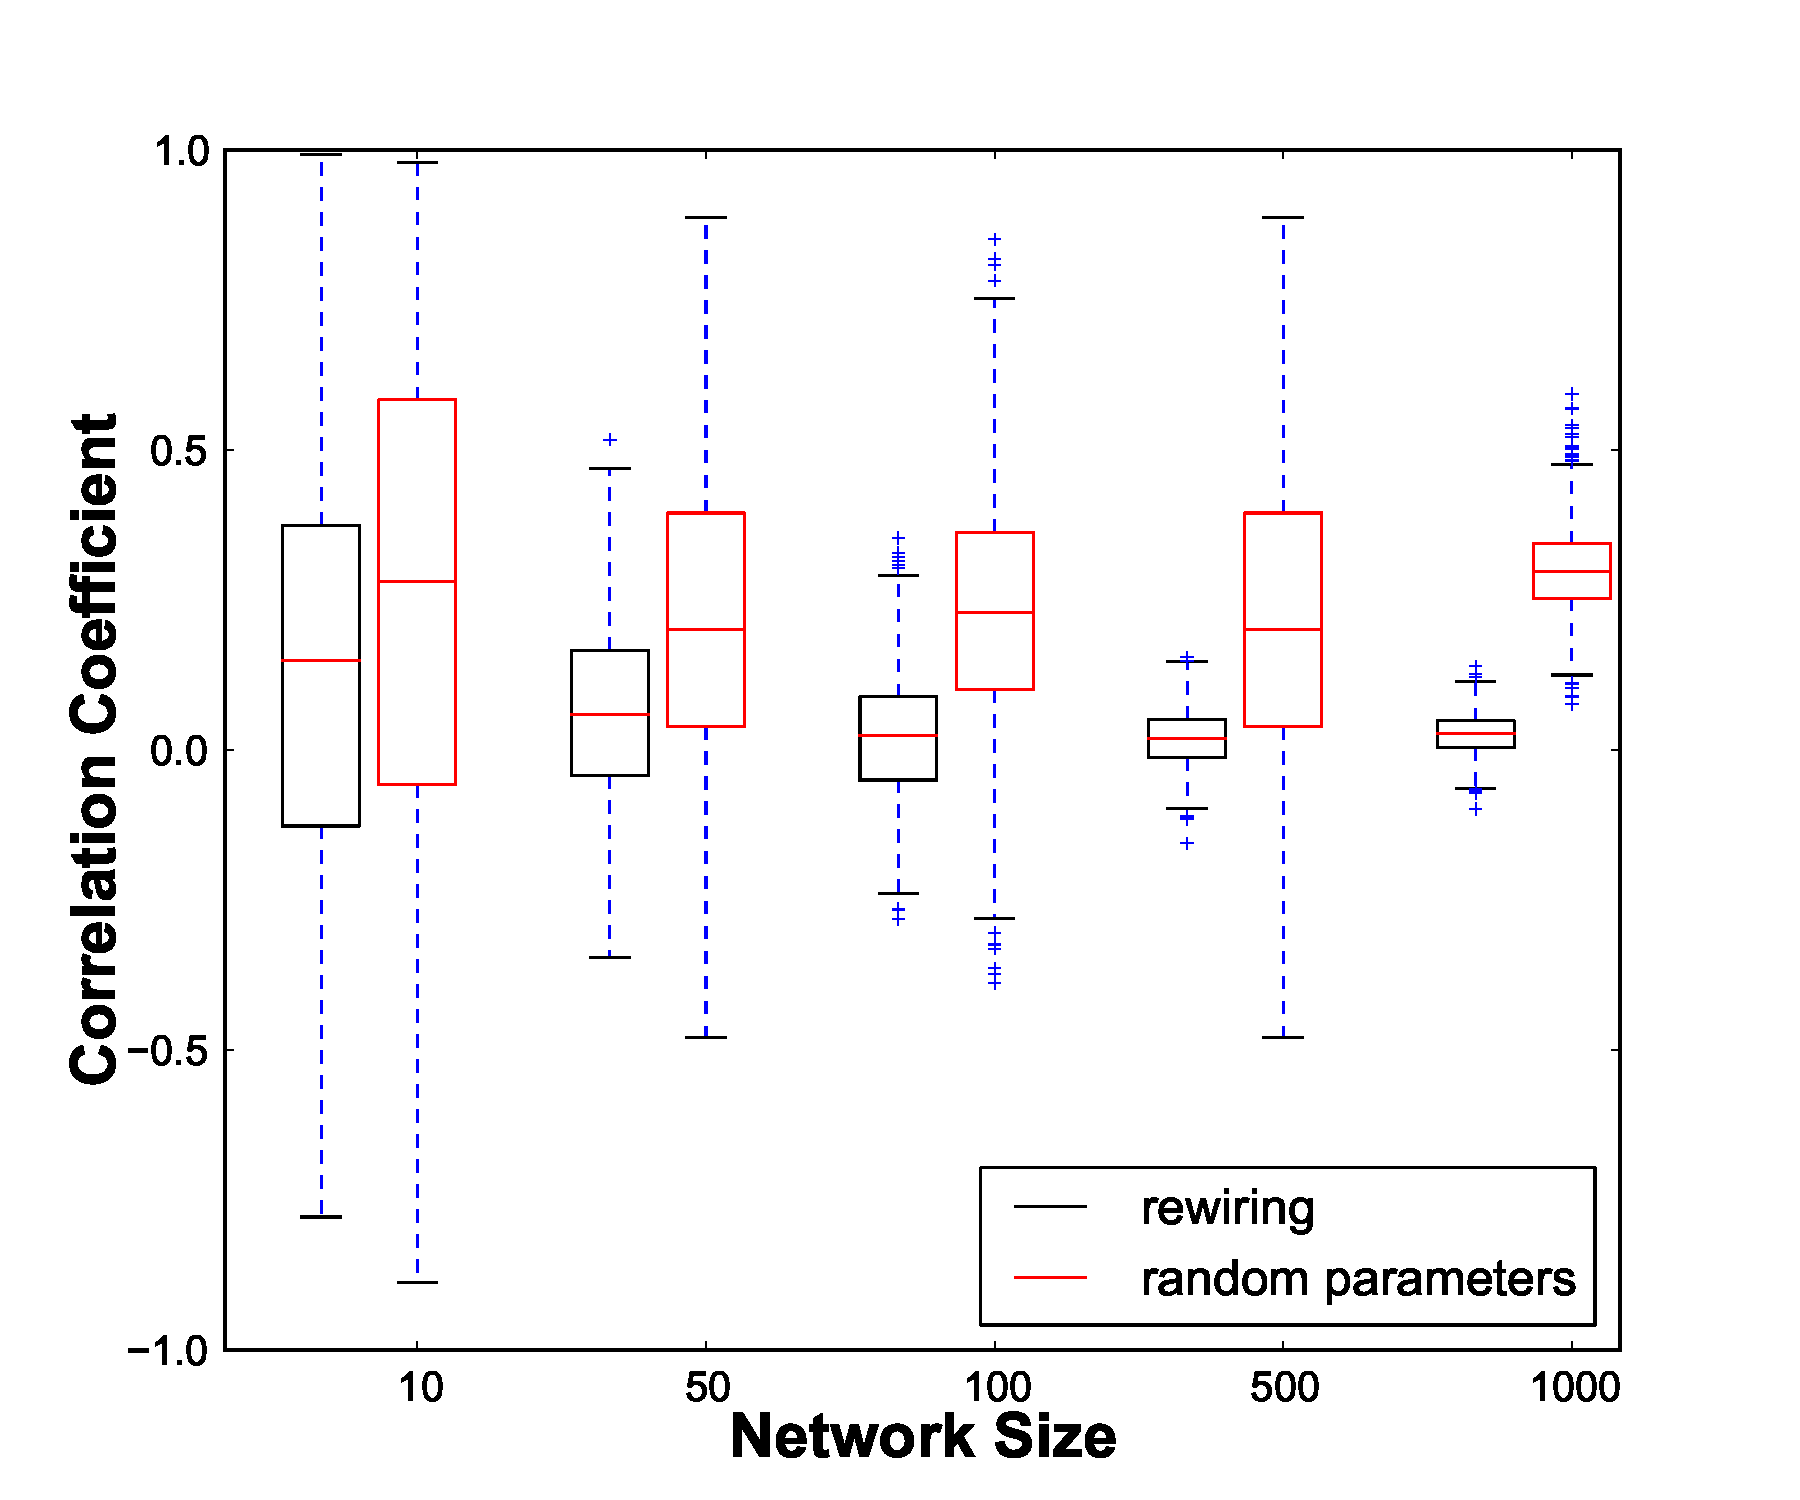
\includegraphics[width=0.45\textwidth]{system_size.pdf}
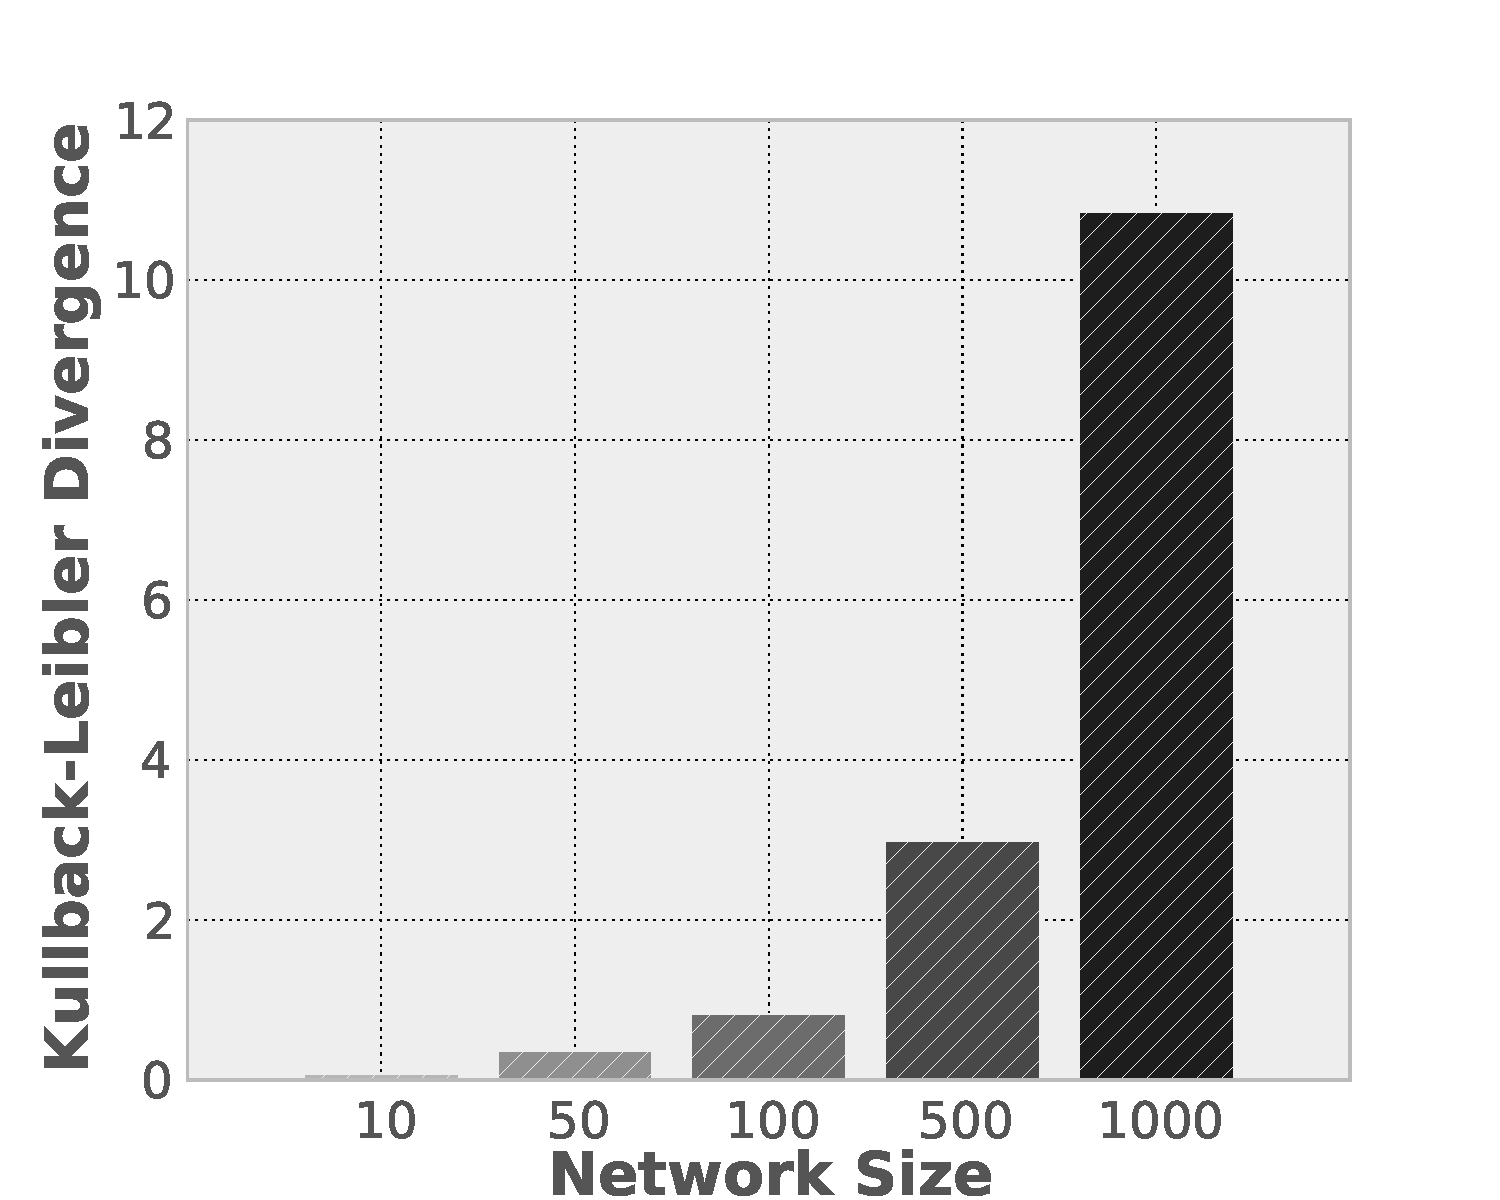
\includegraphics[width=0.45\textwidth]{kl_system_size.pdf}
\end{center}
\caption[Effect of rewiring and parameter change]{
{\bf Effect of network rewiring and kinetic parameter change for different network
sizes.} 
(A) Distribution of the correlation coefficients
before and after rewiring (change of parameters) in black (red) for 
different network sizes. (B) Kullback-Leibler divergence of the 
correlation coefficient distributions in (A) for different network
sizes.
}
\label{fig:system_size}
\end{figure}

One has to keep in mind that when changing the parameters,
the connection strengths of individual edges are also varied,
and only the network connectivity remains the same. Nevertheless,
parameter change has in general a higher correlation coefficient
and thus less effect than rewiring, which changes the connectivity only.
Therefore, the network response pattern changes most dramatically
if and only if the wiring scheme
itself, rather than the connection strengths, is changed.
This result highlights the importance of network topology in
determining the network dynamics, 
since rewiring decreases
the correlation of network response more strongly than 
parameter change, and this effect becomes more pronounced in
larger networks. Our conclusion is very much in line with a 
recent idea of \emph{geometry-controlled kinetics}~%
\citep{Benichou2010}, or the 
initial distance between reactants in compact systems is 
a key parameter and determinant of reaction kinetics, which 
could possibly be applied to the role that topology plays 
in gene regulatory networks.

The existence of topological determinant in network dynamics
further justifies the assumptions of chemical reaction network
theory (CRNT), that is for any network following mass action kinetics,
a non-negative integer $\delta$ called the
deficiency can be derived from the network structure
alone and the number of steady states and the possibility of 
oscillation can be deduced from the deficiency value~\citep{Conradi2005}.

\subsection{Anti-correlation between dynamics and topology}
\label{sec:anti-correlation}
Previous studies~\citep{Lu2007a,Mar2011} have demonstrated a negative
correlation between the connectivity of a gene in the regulatory network
and its expression variance in the context of static disease models.
Here, we aim to address whether this negative correlation also exists 
between the network topology and its dynamic response.

To this end, we characterized the dynamic gene response strengths from 
various microarray studies of primary human keratinocytes, mouse skin
cells, mouse erythrocyte progenitor cells, \emph{E. coli}, yeast and
correlated them with the connectivity of
%\emph{in silico} 
%network models that are used to generate benchmark datasets for the DREAM 
%(Dialogue for Reverse Engineering Assessments and Methods) challenge. 
%The model (\citealp{Marbach2010}) describes gene expression dynamics by the 
%combinatorial regulation of upstream transcription factors. We constructed 
%\emph{in silico} network models (\ref{fig:degree_response_example}) with a predefined topology from 
transcriptional regulatory networks, for example for \emph{E. coli} 
(\citealp{Gama-Castro2008}) 
and \emph{S. cerevisiae} (\citealp{Balaji2006}). In the case of human and
mouse cells, no such comprehensive gene regulatory networks is available
and we thus took the protein-protein interaction network from 
the BioGRID~%
\citep{Stark2006} version 3.1.86 (March 2012) as a first approximation. 
We further investigate the same correlation in a synthetic random,
uniform, small-world, scale-free or bow-tie network. Network dynamics was simulated after 
random 
multi-factorial perturbations from the steady state. 
For both biological and synthetic networks, the response 
strengths of individual genes are quantified by means of multidimensional 
scaling (\ref{sec:response_strength}). 
This workflow enabled us to investigate how the dynamic
response pattern of a network relates to its topology (\ref{fig:degree_response_example}). 

\begin{figure}[!ht]
\begin{center}
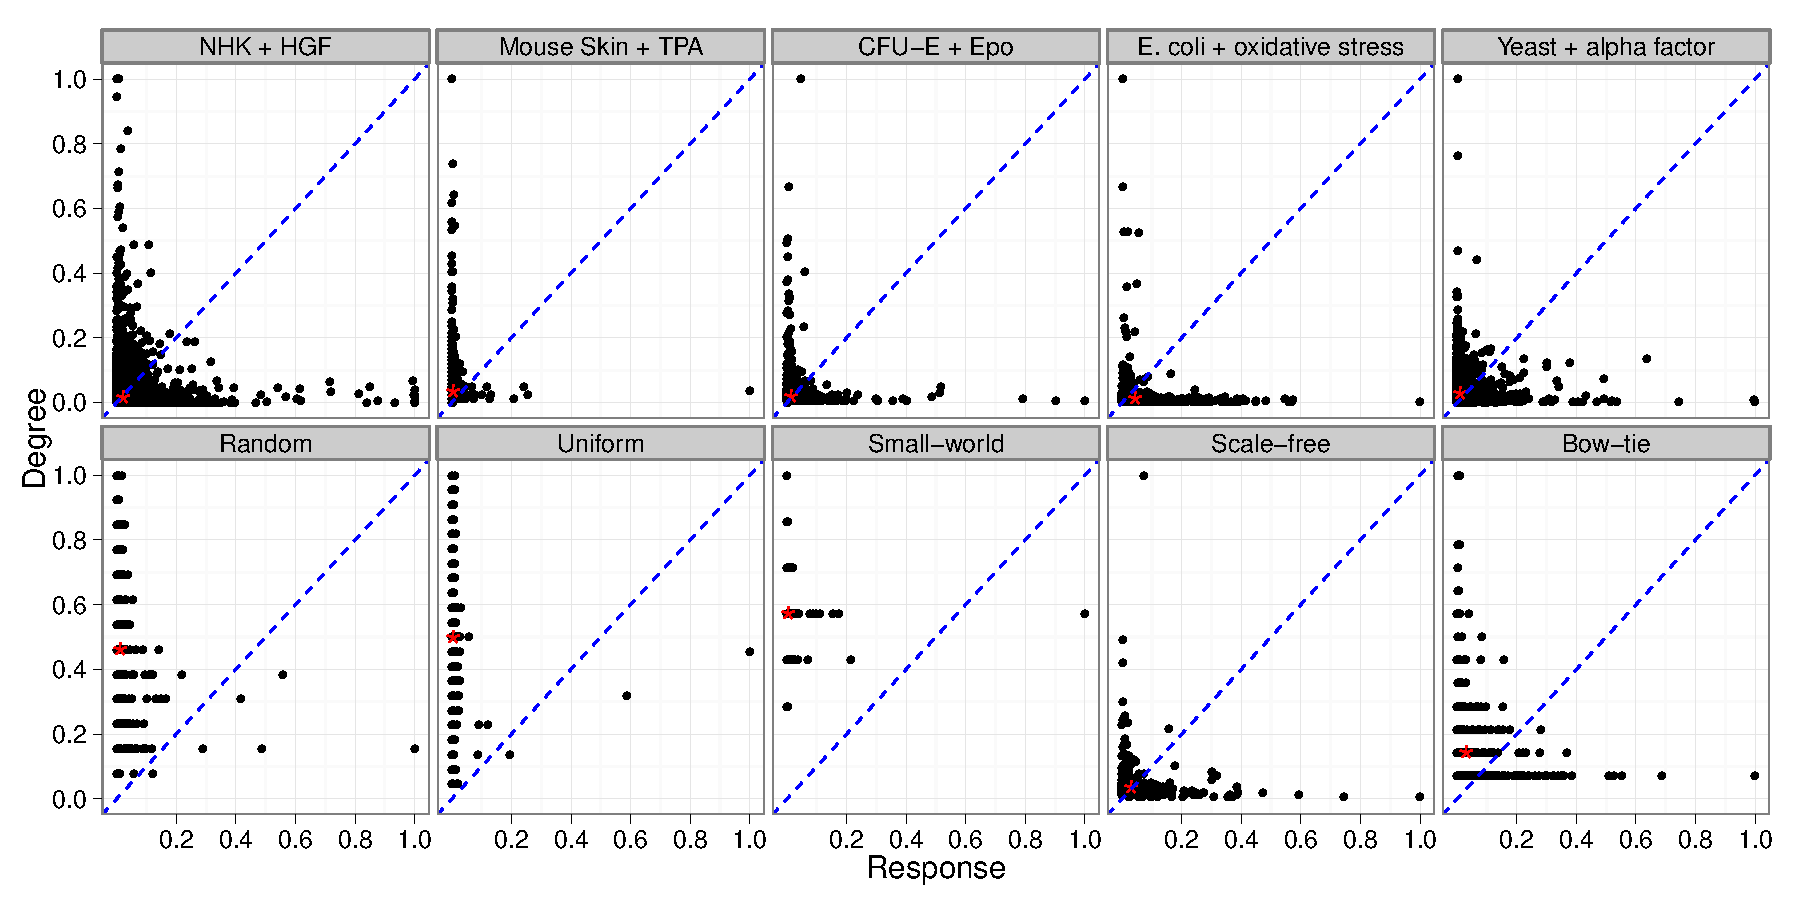
\includegraphics[width=\textwidth]{degree_response-example.pdf}
\end{center}
\caption[Anti-correlation between response and connectivity]{
{\bf Anti-correlation between response and connectivity for biological and 
\emph{in silico} networks.} 
Shown are the correlations between topology and dynamic response for different
biological networks (upper panel) and synthetic \emph{in silico} networks
(lower panel). Blue dashed lines indicate the identity and red asterisks 
represent the centers of mass for each 2-D point distribution.
}
\label{fig:degree_response_example}
\end{figure}

\begin{figure}[!ht]
\begin{center}
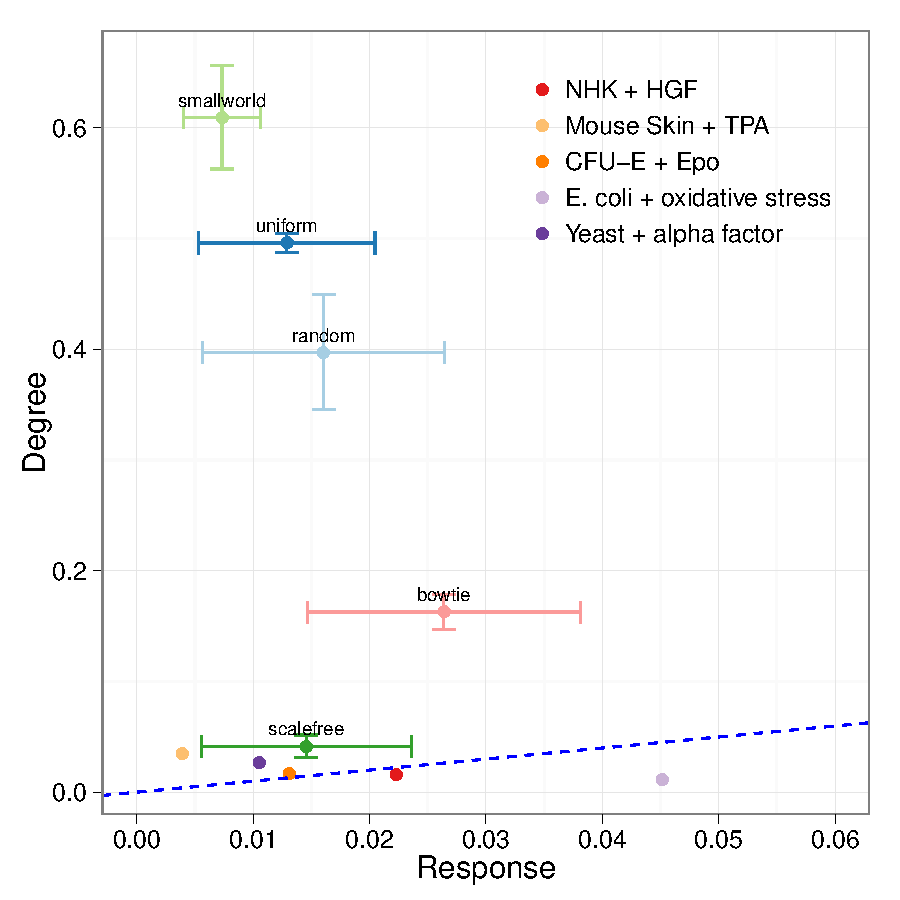
\includegraphics[width=0.8\textwidth]{degree_response-summary.pdf}
\end{center}
\caption[Comparison between biological and \emph{in silico} networks]{
{\bf Centers of mass of the response-connectivity distribution for biological
and \emph{in silico} networks.} 
The point and error bars for \emph{in silico} networks indicate the mean
and standard deviation of 1000 realizations of different networks respectively.
Blue dashed line denotes the identity as in \ref{fig:degree_response_example}.
}
\label{fig:degree_response_summary}
\end{figure}

Our results demonstrated that genes in biological networks with a high level 
of change in expression are more likely to be peripheral nodes 
(low connectivity) in the network, whereas hubs (nodes with higher 
connectivity) and superhubs (nodes that link hubs) tend to have a lower level 
of change in expression. This anti-correlation is less pronounced for  
\emph{in silico} networks to a different degree, as can be seen from the closeness
of the red center of mass to the blue identity line. By characterizing the 
anti-correlation using the center of mass for each point distribution, we
can show that scale-free\footnote{Although this result should be interpreted 
with caution according to \ref{sec:scale_free}.} and bow-tie networks are more closely related to
biological networks, whereas random, uniform and small-world networks behave
differently (\ref{fig:degree_response_summary}).

\subsection{Topology and perturbation together shape the network dynamics}

\begin{figure}[!ht]
\begin{center}
\includegraphics[width=\textwidth]{degree_response-deg_dist.pdf}
\end{center}
\caption[Combination of topology and perturbation]{
{\bf Comparisons of the connectivity-response pattern.} 
Comparison of the connectivity-response
anti-correlation for different network topologies and
perturbation schemes. norm: normally distributed perturbation
factor, max: perturb all genes to the maximum level of 1 at
the initial time point, rank: perturbation strength
proportional to the node degree (hubs more strongly
perturbed).
Blue dashed lines indicate the identity and red asterisks 
represent the centers of mass for each 2-D point distribution.
}
\label{fig:degree_response_deg_dist}
\end{figure}

In order to determine the driving force behind the ubiquitous
anticorrelated pattern between response strength and connectivity, we
further investigated different combinations of the network topology and
external stimulation schemes and how they affect the network response
pattern (\ref{fig:degree_response_deg_dist}). 
The scale-free networks with both the \emph{norm} and \emph{max}
perturbation strategies resemble the connectivity-response pattern of 
biological networks most closely (cf. \ref{fig:degree_response_example}), 
as can be seen from both centers of mass
lying closely to the diagonal. In the case of \emph{rank} perturbation,
although the center of mass remains at the bottom left corner, the node
connectivity and its response strength clearly show a positive correlation,
which stands out from the remaining networks. 

\begin{figure}[!ht]
\hskip 0.5in A \hskip 2.5in B
\begin{center}
\includegraphics[width=0.45\textwidth]{degree_response-ks2d_hgf_clustered.pdf}
\includegraphics[width=0.45\textwidth]{degree_response-ks2d_yeast_clustered.pdf}
\end{center}
\caption[Comparison of the synthetic and biological networks]{
{\bf Similarity between the topology/perturbation combination and the 
biological networks.} 
(A) Kolmogorov-Smirnov distances between each
network/perturbation combination and the real microarray
data from keratinocytes stimulated with HGF, the smaller
the KS distance, the more closely related it is between
biological and synthetic networks. We infer that the human
gene regulatory network is mostly reminiscent of the
scale-free network with normally distributed perturbation
applied.
(B) Kolmogorov-Smirnov distances between each
network/perturbation combination and the real microarray
data from yeast cells synchronized with the alpha factor,
the smaller
the KS distance, the more closely related it is between
biological and synthetic networks. We infer that the yeast
gene regulatory network has both the scale-free and bow-tie
feature.
}
\label{fig:degree_response_ks2d}
\end{figure}

This combined topology and perturbation feature also seems to be highly
species dependent. Here we quantify the similarity between synthetic
and biological networks by defining a 2-D Kolmogorov-Smirnov distance~%
\citep{Press2007}
between the connectivity-response distributions.
While the human keratinocyte stimulated with HGF is
most closely related to the scale-free network with the normally distributed
perturbations (\ref{fig:degree_response_ks2d}), the yeast cell synchronized
with the alpha factor tends to behave in a way close to both scale-free and
bow-tie networks.

Taken together, it is 
biologically more plausible that cellular interaction 
networks are perturbed by a normally
distributed factor upon external stimulation, where most of the genes are
untouched and few of them are triggered to the level either above or
below the steady state. The \emph{max} and \emph{rank} perturbation scenario, however, 
seem more restrictive and hard to be implemented by the cell.

\begin{figure}[!ht]
\begin{center}
\includegraphics[width=\textwidth]{degree_response-rf.pdf}
\end{center}
\caption[Node feature importance]{
{\bf Node feature importance in networks with different topologies and 
perturbations.} 
Normalized node feature importance as calculated by a random forest regression
with response strength as the dependent variable. Errorbars show the mean 
importance and the standard deviation of 1000 random forest runs.
The features are: \emph{perturb}, perturbation factor; \emph{in.deg.act},
activating in-degree; \emph{in.deg.inh}, inhibiting in-degree;
\emph{out.deg.act}, activating out-degree; \emph{out.deg.inh},
inhibiting out-degree; \emph{delta}, decay rate, related to the half-life
by $\delta = \ln 2 / \tau_{1/2}$; \emph{k.mean}, mean dissociation constant
of all incoming connections; \emph{n.mean}, mean Hill coefficient of all
incoming connections.
}
\label{fig:degree_response_rf}
\end{figure}

To systematically determine the relative contribution
of topology, perturbation and kinetic parameters to the network response,
we performed a random forest regression with the response strength as the
dependent variable and all other node parameters as independent variables.
The random forest regression is a robust and unbiased 
approach that is based on an ensemble of decision trees.
It has been shown to perform extremely well across large 
classes of data~\citep{Caruana2008} and generates, among
other things, a ranking of feature variables by their 
explanatory power. More specifically, we applied a variant
of random forest that
takes multiple subsamples of the data without replacement and
tries to build an ensemble of conditional inference trees~\citep{Strobl2007}. At each node (step), a conditional inference tree
chooses an independent variable to split the dataset, based on a univariate $p$-value from a permutation
independence test between the independent and dependent variables. We randomly sample 5 candidate
input variables to split at each node, and set the number of trees to be 1000, which is well above our
number of variables.
We calculate the variable importance for each feature as the mean decrease in accuracy after permuting a specific input variable, the number of permutations is fixed to 3.

In the case of the \emph{norm} and \emph{max} perturbations
(\ref{fig:degree_response_rf}), 
both the perturbation factor and the connection weights as represented by
the Hill coefficient (\emph{n.mean}) and the dissociation constant 
(\emph{k.mean}) play a predominating role in predicting the network dynamics.
When applying the \emph{rank} perturbation, in contrast, it is the network
connectivity as characterized by the in-/out-degrees and the connection weights
that explain the network dynamics well. The kinetic parameter, decay rate,
does not have a high importance score for any combination of network
topology and perturbations.

This result cross-validates and adds new information to 
the observation in 
\ref{sec:topology_kinetics}, namely network connectivity is
more important than kinetic parameters in determining the 
dynamic response. Apart from connection strength, which is 
affected in
both rewiring and change of parameters, the importance of 
node degrees is hardly higher than that of kinetic parameters.
Taking into account that rewiring has a significantly larger
effect on dynamics than kinetic parameters, it is clear that
network topology cannot be explained only by node degrees,
which is a local topological metric 
(\ref{sec:topology_definition}). Furthermore, the random
forest regression approach underscores the important role of 
perturbation 
as a new parameter dimension, which is not investigated in
the rewiring/parameter change experiment.
Altogether, we conclude that
network topology alone, especially node degrees, is the 
critical parameter in the \emph{rank} perturbation scenario, 
and the combination of both perturbation and topology shapes
network dynamics in a more common setting.

\subsection{Strong regulators correlated with the phenotype}
\label{sec:strong_regulator_phenotype}
The fact that strongly regulated genes always have a low degree and thus are
located at the periphery of the network poses the question whether these genes
mediate the computation of the whole network and then translate it into the 
phenotype. To address this question, we took the transcriptome data from the literature,
where time-resolved responses of \emph{E. coli} (\citealp{Jozefczuk2010}) and 
\emph{S. cerevisiae} (\citealp{Spellman1998,Cho1998}) are
measured under different stimuli. We found a similar anti-correlation between
network topology and response in the above datasets (\ref{fig:ecoli_yeast_go} A,C). Furthermore, we
carried out the enrichment test of Gene Ontology (GO) terms in the significantly 
strong responders identified from MDS. 
For \emph{E. coli} cells in response
to different stress conditions (\ref{fig:ecoli_yeast_go} D), GO terms such as 
locomotion, flagella organization
are over-represented in the strongly responding genes, which is in accordance
with the fact that flagella motility requires a steep proton gradient between 
the periplasmatic space and the cytoplasm, a change in cell motion could 
indicate energy deficiency resulting from the environmental stress~\citep{Jozefczuk2010}. 
On the other hand, for yeast cells in response to different synchronization
treatments (\ref{fig:ecoli_yeast_go} B), GO terms like cell cycle, cell division, cytokinesis are more 
enriched than expected among strong responders, which is also in line with the
phenotype of cell cycles. Taken together, we found strongly induced genes, 
which are located at the periphery of gene regulatory networks, are nicely
correlated with the cellular phenotype.

\begin{figure}[H]
\begin{center}
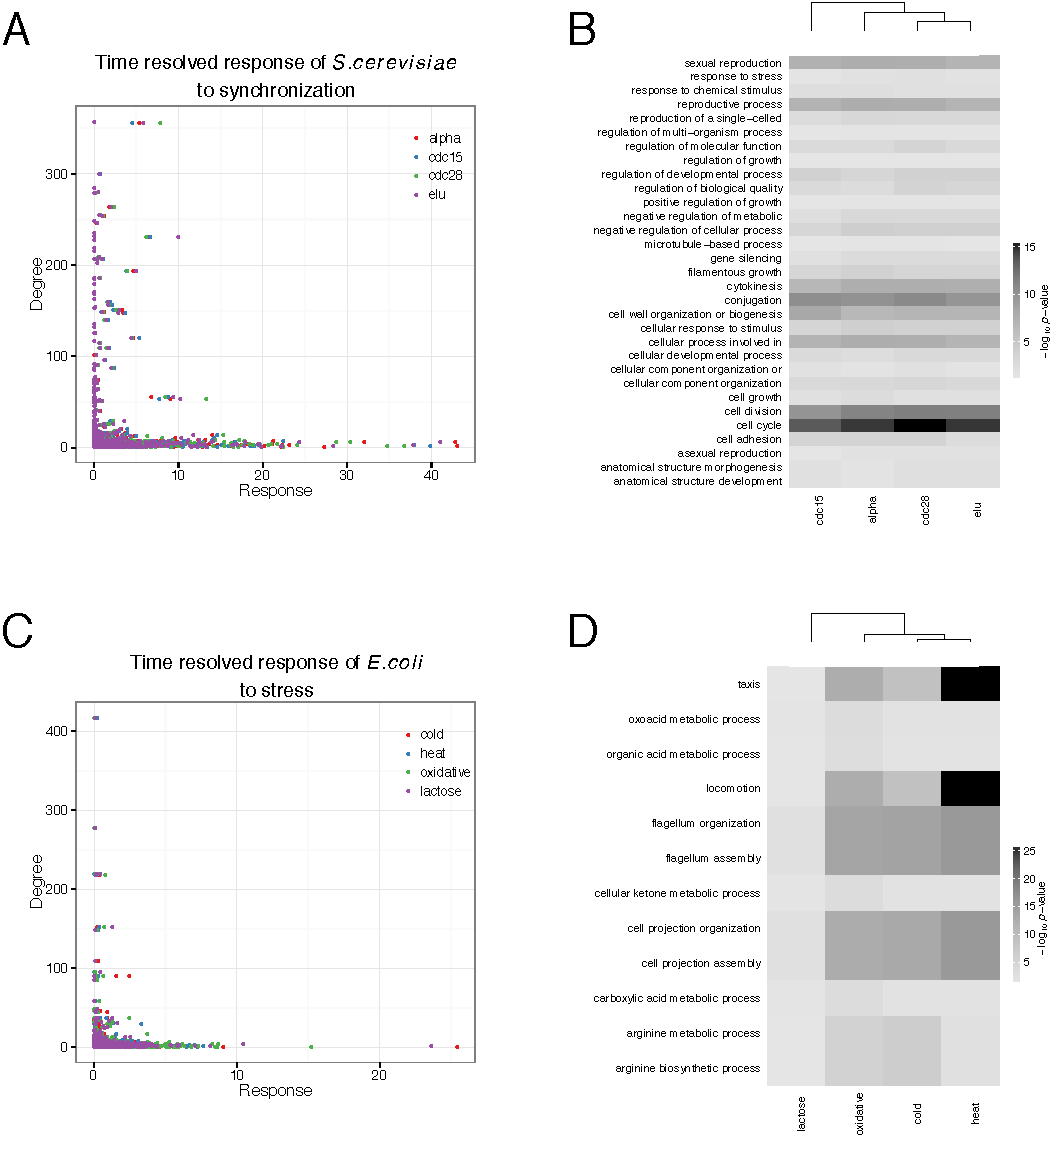
\includegraphics[width=\textwidth]{yeast_ecoli_go.pdf}
\end{center}
\caption[GO term enrichment of strongly regulated genes]{
{\bf Strongly regulated peripheral genes are correlated with the phenotype.}
(A) Topology-response
anti-correlation of \emph{S. cerevisiae} in response to different synchronizations
(extracted from \citealp{Spellman1998,Cho1998}). 
(B) Enrichment of GO
terms in the strongly induced (response strength $> -\log_{10}0.05$) 
peripheral genes of \emph{S. cerevisiae}. Shown 
are $p$-values
from Fisher's exact test in gray scale for different GO terms under different 
conditions.
(C) Topology-response anti-correlation of \emph{E. coli} in response 
to different stresses (extracted from \citealp{Jozefczuk2010}). 
(D) Enrichment of GO terms
in the strongly induced (response strength $> -\log_{10}0.1$) 
peripheral genes of \emph{E. coli}. Shown are $p$-values
from Fisher's exact test in gray scale for different GO terms under different 
conditions. 
}
\label{fig:ecoli_yeast_go}
\end{figure}


\begin{figure}[!ht]
\begin{center}
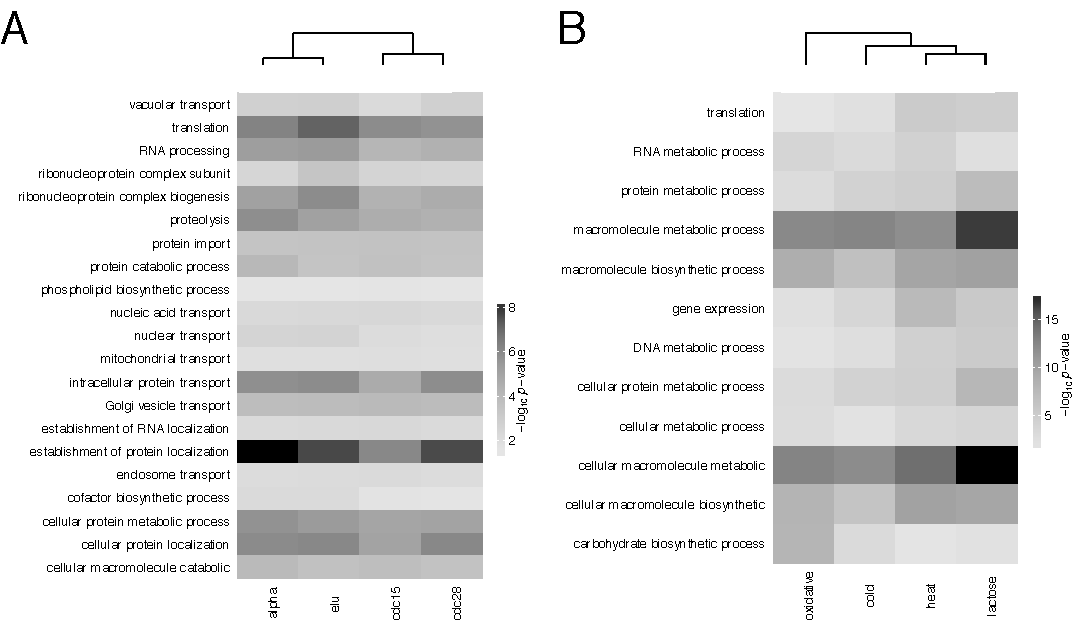
\includegraphics[width=\textwidth]{yeast_ecoli_go_under.pdf}
\end{center}
\caption[GO term depletion of strongly regulated genes]{
{\bf Metabolic and transcriptional regulation is under-represented in 
strongly regulated peripheral genes.}
(A) Under-representation of GO
terms in the strongly induced (response strength $> -\log_{10}0.05$) 
peripheral genes of \emph{S. cerevisiae} from
the dataset in \ref{fig:ecoli_yeast_go}. Shown 
are $p$-values
from Fisher's exact test in gray scale for different GO terms under different 
conditions.
(B) Under-representation of GO terms
in the strongly induced (response strength $> -\log_{10}0.1$) peripheral genes 
of \emph{E. coli} from the dataset 
in \ref{fig:ecoli_yeast_go}. Shown are $p$-values
from Fisher's exact test in gray scale for different GO terms under different 
conditions. 
}
\label{fig:ecoli_yeast_go_under}
\end{figure}

Our results present an invariant feature of gene regulatory
networks, namely strongly responding genes correlate with
the phenotype and constitute sparsely connected peripheral nodes.
In contrast, densely connected hub genes are only moderately
regulated. Further GO term analysis reveals that metabolic
function and transcriptional regulation are depleted in the
strong responders (\ref{fig:ecoli_yeast_go_under}).
This feature can be considered in light of 
the microarray data analysis that only attempts to obtain
a ranked list of genes~%
\citep{Boulesteix2009,Smyth2004}. On the one hand, different ranking
algorithms often lead to unreproducible lists; On the other
hand, if one only examines those top-ranked genes in more
details, one only focuses on the genes related to the phenotype,
or workhorses, and will thus not be able to detect master regulators
that determine the mechanism of action.

The finding of strongly regulated genes being sparsely connected
has also implications for the reverse engineering of gene regulatory
networks. Although sparsity has widely been assumed in the field
of reverse engineering~\citep{Yeung2002,Gardner2003}, especially
for solving linear ordinary differential equation models, it was
not explicitly stated whether this assumption holds. From what
we learned so far, if one starts to reconstruct the network consisting only of
differentially regulated genes, it is also highly likely that
the network is sparse.

The importance of peripheral nodes in the networks has recently been addressed~%
\citep{Sikic2011}, in which the authors developed a new epidemic centrality
metric to assess the epidemic impact of each node in the disease spreading
network. This metric takes into account both the structural and 
the dynamic properties of the node. As a result,
it has been shown that the epidemic centrality of structually peripheral nodes is 
comparable to that of the central nodes with high degree, k-cores value or 
betweenness. This study underlines the prominent role played by peripheral
nodes, which, according to our results, can also be critical in the 
development of cellular phenotypes.

\section{Biological application}
We further went on to verify our hypothesis that strongly regulated peripheral 
genes are correlated with the phenotype by means of an \emph{in vitro}
mammalian cell system, namely migration of primary human keratinocytes extracted from the foreskin
upon the treatment of hepatocyte growth factor (HGF). 
This system is of particular interest to wound healing, which is a complex 
dynamic process involving a variety of players in the skin.
HGF activates its receptor MET, a proto-oncogene commonly mutated in 
metastasizing epithelial cell, and thus the cellular response to HGF is 
crucial for understanding the migration behavior or even wound healing and 
metastasis in general. 

We measured
the gene expression profiles in keratinocytes up to 8h after treatment of HGF (\citealp{Busch2008}) 
and identified
key genes with a large response strength according to MDS 
(\ref{fig:degree_response_hgf}). 
In the figure, we highlighted 2 example hub genes, TGFBR1
and EGFR, and 8 top responders. It is again confirmed that
hub genes that are strongly cross-linked in the signalling
network are only moderately expressed. In contrast, the
strongly expressed top responders all have a low 
connectivity.
The gene list 
ranked by MDS-based response metric largely agrees with a previous list 
according to the ranking of peak and mean fold expression over time~%
\citep{Busch2008}. Among the top-ranked genes, PTGS2 is a prostaglandin 
synthase and a major mediator of inflammation; AKAP12 is a regulator 
of protein kinase A (PKA) signaling, which could suppress HGF-induced 
migration; PLAUR encodes the plasminogen urokinase activator receptor;
CEACAM1 encodes a member of the immunoglobulin superfamily and is a
cell adhesion molecule in leukocytes, epithelial and endothelial cells.
HBEGF is an EGF-like ligand to the EGF receptor, which itself mediates $cjun$-dependent formation of the keratinocyte leading edge and is also an important player during tumor development and progression~\citep{Busch2008}.
As an \emph{in vitro} verification, the scratch assay is performed
where the monolayer keratinocytes were damaged with a \emph{scratch} using a pipette tip
and HGF and the respective inhibitors (\ref{table:inhibition_method}) 
of strong regulators are added to 
the medium. The migration phenotype was then assessed by the closed
area after a certain period of time between two cell fronts across the \emph{scratch}.
It has been shown that the perturbation of all the above players can reduce the closed migration 
area, thus inhibiting the cellular phenotype~\citep{Busch2008,Schnickmann2009}.

\begin{figure}[!ht]
\begin{center}
\includegraphics[width=\textwidth]{degree_response_hgf_modified.pdf}
\end{center}
\caption[Degree-response anti-correlation of HGF-induced response]{
{\bf Degree-response anti-correlation of gene regulation in HGF-stimulated
keratinocytes.}

}
\label{fig:degree_response_hgf}
\end{figure}

We further identified 3 genes that only show in the MDS-based ranking.
FERMT2 is also called kindlin 2 and participates in the connection between 
extracellular matrix (ECM) adhesion sites and the actin cytoskeleton, the
colocalization of kindlin gene products is relevant for the pathophysiology
of the Kindler syndrome; Interleukin 8 is one of the major mediators
of the inflammatory response; PTGER4 is a receptor for prostaglandin E2.
The functions of these genes all point to the regulation of cell shape and
inflammation. 
To verify the role these genes play in keratinocyte migration,
we used either antibodies or siRNAs to perturb the products of these genes
(\ref{table:inhibition_method}). One example is shown in 
\ref{fig:scratch_assay}, where keratinocytes treated with HGF and IL8 
neutralizing antibodies were found to migrate slower after 12 hours 
than those only treated with HGF.
Indeed, the inhibition of FERMT2, IL8 and PTGER4 all have an effect on the 
migratory phenotype of keratinocytes, and the relative migration inhibition
by their inhibitors
closely matches the response strength of these genes
(\ref{fig:migration_prediction}). In summary, the more strongly a gene
is regulated, the more closely related it is to the phenotype.

\begin{longtabu} to \textwidth {X[c]X[c]X[c]}
\caption[Inhibitors of key players]{
Key regulators as identified by the MDS-based response
metric, their inhibitors and Gene Ontology terms.} \\
\hline
\textbf{Key players} & \textbf{Inhibition} & \textbf{Function (GO analysis)} \\
\hline
\endhead
\rowcolor{Gray} PTGER4 &  L-162982 & immune response; G-protein coupled receptor signaling pathway \\
PLAUR & neutralizing antibody \citep{Schnickmann2009} & chemotaxis \\
\rowcolor{Gray} IL-8 & neutralizing antibody &  angiogenesis; inflammatory response \\
PTGS2 & meloxicam \citep{Busch2008} & prostaglandin biosynthetic process  \\
\rowcolor{Gray} FERMT2 &  siRNA &  cell adhesion; regulation of cell shape \\
AKAP12 &  perturbation of protein kinase A \citep{Busch2008} &  positive regulation of protein kinase A signaling cascade  \\
\rowcolor{Gray} CEACAM1 & siRNA \citep{Schnickmann2009} &  angiogenesis; integrin-mediated signaling pathway  \\
HBEGF & GW2974, double specific inhibitor of EGFR \citep{Busch2008} &  epidermal growth factor receptor binding; heparin binding  \\
\hline
\label{table:inhibition_method}
\end{longtabu}
%\newpage

\begin{figure}[!ht]
\begin{center}
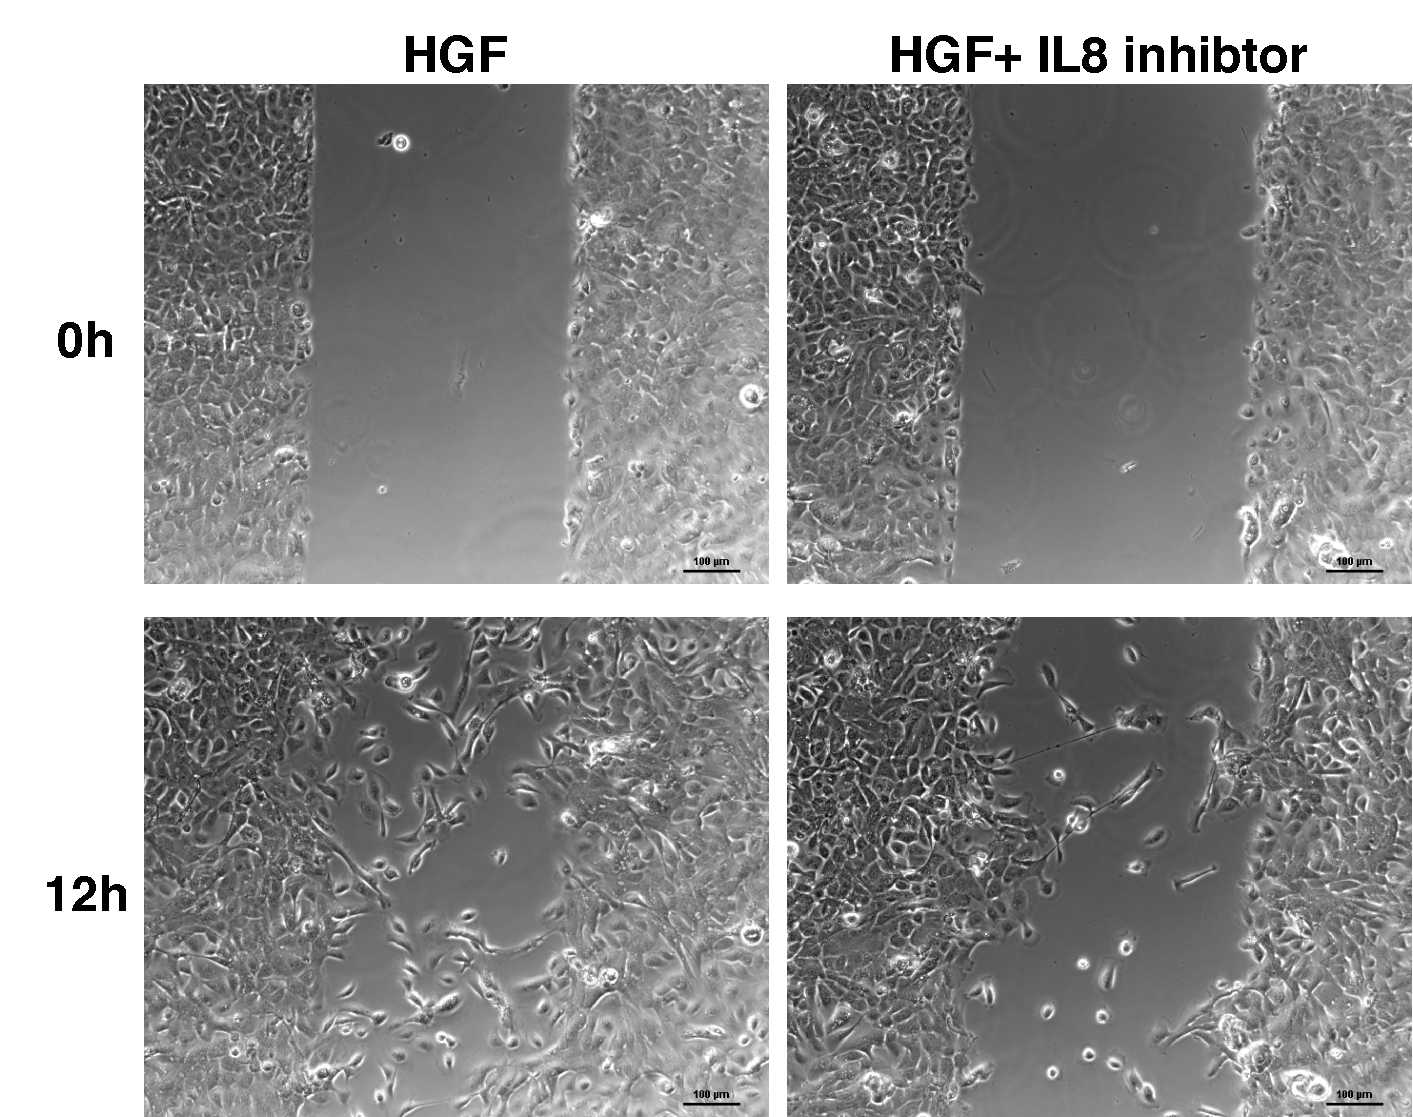
\includegraphics[width=\textwidth]{scratch_assay.pdf}
\end{center}
\caption[Migration of keratinocytes]{
{\bf Comparison of keratinocyte migration under the control condition and 
inhibition of IL8.}
Time-lapse microscopy of keratinocytes treated with HGF and the IL8 inhibitors. 
Control keratinocytes were treated with HGF alone. Images recorded on a Nikon 
microscope and an ibidi humidity chamber.
}
\label{fig:scratch_assay}
\end{figure}

\begin{figure}[!ht]
\begin{center}
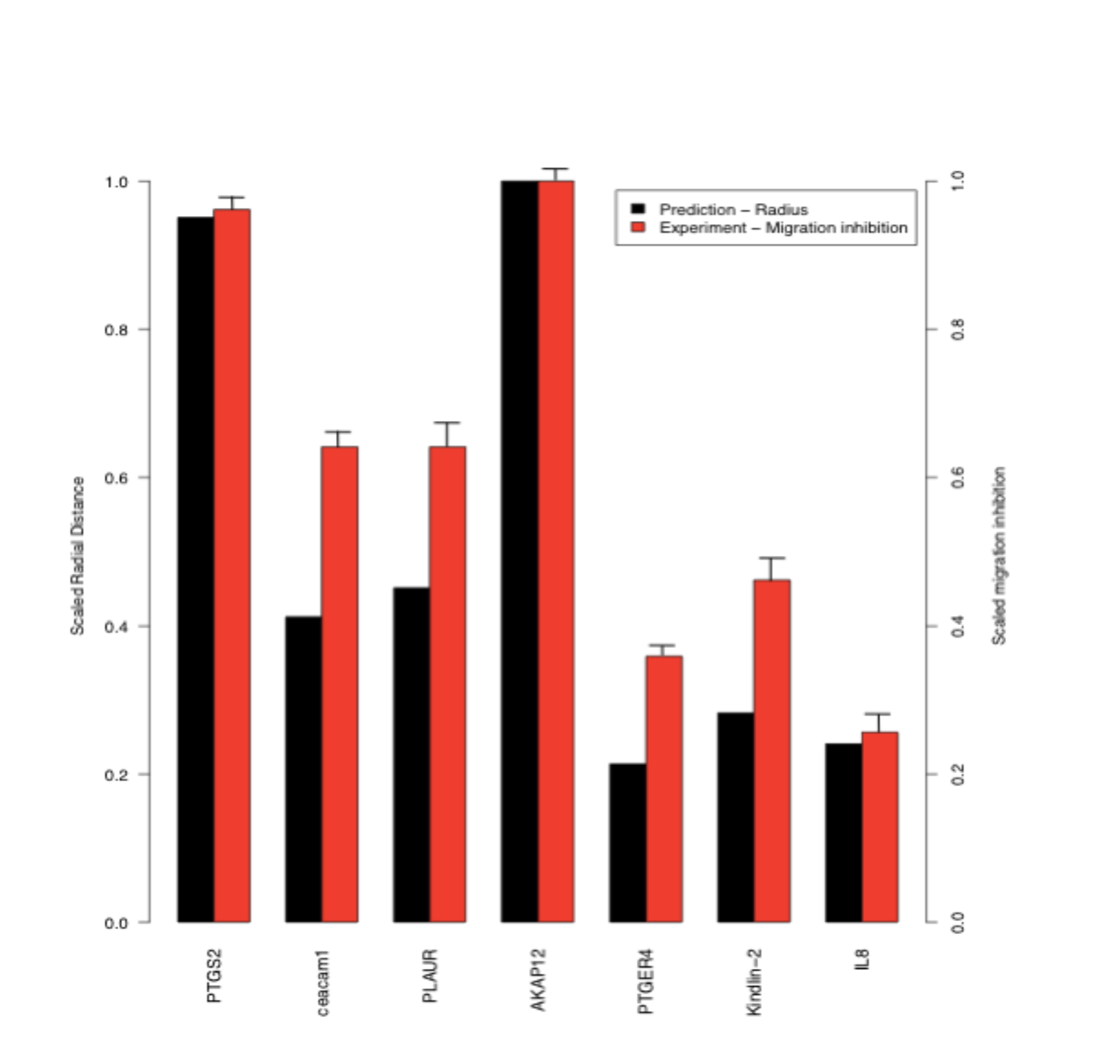
\includegraphics[width=0.9\textwidth]{migration_prediction.pdf}
\end{center}
\caption[Prediction of migration inhibition after perturbing key players]{
{\bf Prediction of migration inhibition after perturbing key players identified
from MDS.} 
}
\label{fig:migration_prediction}
\end{figure}

The multidimensional scaling-based response score also has
its limitations, as can be seen from the deviation between
the predicted and the measured migration inhibition in 
\ref{fig:migration_prediction}. First, the response metric
derived from the transcriptome data might not correspond
well to the protein-level regulation, which in the end 
determines whether the key player inhibitors have an effect
or not. Second, it is always compression or loss of information
to collapse the time-resolved transcriptome response into
a single score. The response metric is thus aggregated over
time, and what it cannot tell is, for instance, when to 
inhibit a certain gene.

Nevertheless, we provided a proof of principle that key genes with a high MDS-based response
score are correlated with the cellular phenotype, as the inhibition of them
leads to a reduced phenotypical outcome.
The top responders fulfil their functions
while being located at the periphery of the network and sparsely connected.
The advantage of the MDS-based response metric is that it can rapidly generate
testable hypotheses from the multidimensional gene expression time series data.

